\documentclass[conference]{IEEEtran}
\usepackage{enumitem}
\usepackage[document]{ragged2e}
\usepackage{blindtext}
\usepackage{graphicx}
\usepackage{float}
\usepackage{amsmath}
%\usepackage{natbib}
\usepackage{cite}
\usepackage{lipsum}

\graphicspath{ {./}{./images/} }

\title{Joint Radar Communication System using OFDM}

\author{

\IEEEauthorblockN{Owen Sowatzke}
\IEEEauthorblockA{\textit{Electrical Engineering Department} \\
\textit{University of Arizona}\\
Tucson, USA \\
osowatzke@arizona.edu}

\and
\IEEEauthorblockN{Iman Miraki}
\IEEEauthorblockA{\textit{Electrical Engineering Department} \\
\textit{University of Arizona}\\
Tucson, USA \\
imanmiraki@arizona.edu}}

\begin{document}


	\raggedbottom
	\maketitle
	%\twocolumn[
	%\begin {@twocolumnfalse}
	
\begin {abstract}


This paper explores the integration of radar and communication systems using a Joint Radar-Communication (JRC) framework based on Orthogonal Frequency Division Multiplexing (OFDM). By leveraging OFDM waveforms for both radar sensing and data communication, the proposed system achieves enhanced spectrum utilization, reduced hardware complexity, and efficient resource sharing. The JRC design incorporates zero-forcing techniques to generate Range-Doppler Matrices (RDMs) from OFDM returns, enabling accurate radar sensing while maintaining high communication capacity. Simulation results demonstrate that the system provides comparable radar resolution and communication performance to standalone implementations, with notable advantages in dynamic range and sidelobe suppression. Additionally, parameter adjustments optimize radar detection for varying target distances and velocities, achieving reliable operation up to 700 meters. These results highlight the potential of JRC systems for modern vehicular and multi-functional applications where sensing and communication coexist seamlessly.


\end{abstract}



\section {Introduction}
     Vehicle-to-Vehicle (V2V) networks seek to enhance road safety and reduce traffic congestion by sharing road and traffic information between vehicles in real time. To avoid delays associated with third party networks, vehicle-to-vehicle communication systems need dedicated bandwidth. Instead of wasting additional spectrum resources, joint radar communication (JRC) systems attempt to integrate radar and communication systems. This results in reduced bandwidth usage and reduced power consumption while eliminating the need for additional hardware.
     
     In this paper, we design a JRC system, which uses OFDM for communication and zero-forcing to generate a range response from the OFDM returns. Next, we examine the performance of this system and compare it to standalone radar and standalone OFDM implementations.
        
  \section {Radar}
   \subsection {Background}
   
In this section, we provide background on frequency-modulated continuous wave (FMCW) radar, which is used in many automotive applications. FMCW radar continuously transmits a signal whose frequency varies linearly over time (chirp). It measures the time delay between the transmitted and the reflected signals (echoes) to determine the distance of reflecting objects. It can also determine the relative velocity of these objects, by measuring frequency shifts caused by the doppler effect.

	\begin{figure}[H]
    		\centering
    		\fbox{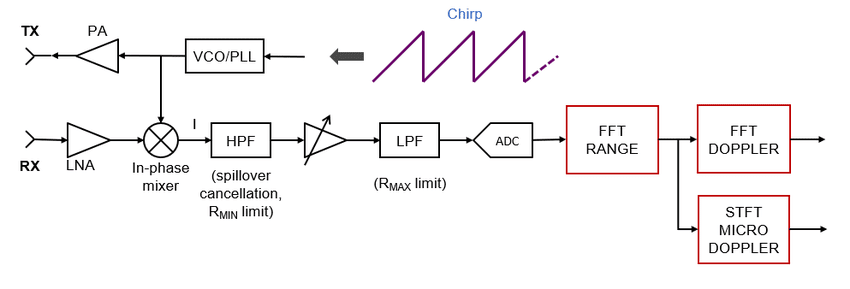
\includegraphics[width=0.9\linewidth]{FMCW Blockdiagram}}
    		\caption{Typical FMCW Block Diagram \cite{9613183}}
    		\label{fig::fmcw_radar}
	\end{figure}
	
 The block diagram shown in Figure \ref{fig::fmcw_radar} depicts the signal processing chain of a typical FMCW radar system. The transmitter generates a frequency-modulated chirp signal of the following form:
 
 	\begin{equation}
 		x(t) = e^{j\pi{\beta}t^2/\tau}
 		\label{eq::chirp}
 	\end{equation}
 	
 	where $\beta$ is the chirp bandwidth and $\tau$ is the chirp duration.
 	
	It transmits this signal out of the antenna towards objects of interest. The receiver receives reflections from each of these objects, which are passed through a low noise amplifier. For each return, the received signal will be a chirp waveform with a frequency offset as illustrated below.
	
	\begin{equation}
		r(t) = e^{j\pi{\beta}(t - t_0)^2/\tau} = e^{j\pi{\beta}t^2/\tau}e^{-j2\pi({\beta}t_0/\tau)t}e^{j\pi{\beta}t_0^2/\tau}
		\label{eq::delayed_chirp}
	\end{equation}
	
	We can mix the received signal with the transmitted signal to create a tone for each return. The frequency of this tone will be proportional to its delay.
	
	\begin{equation}
		f = \frac{{\beta}t_0}{\tau} \Rightarrow t_0 = \frac{{\tau}f}{\beta}
	\end{equation}
	
	The delay of this return is then related to the range of the reflecting object as follows:
	
	\begin{equation}
		R = \frac{ct_0}{2}
	\end{equation}
	
	The relationship between the transmitted and received chirps signals is illustrated below:
	
	\begin{figure}[H]
    		\centering
    		\fbox{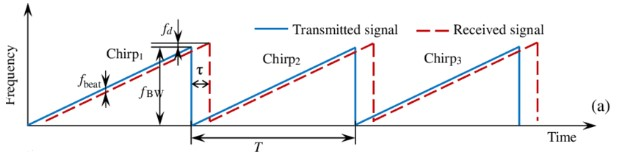
\includegraphics[width=0.8\linewidth]{FMCW Freq-Time graph}}
    		\caption{Plot of Transmit and Receive Signal Frequency vs Time.\cite{Long2019AssistingTV}}
    		\label{fig::fmcw_spectrogram}
	\end{figure}
	
	Note that the chirp bandwidth $\beta$ given in Equation (\ref{eq::chirp}) is inversely proportional to the range resolution ${\Delta}R$.
	
	\begin{equation}
		{\Delta}R = \frac{c}{2\beta}
		\label{eq::range_resolution}
	\end{equation}
	
	Because fine range resolution is desired, $\beta$ is typically very large (on the order of 150MHz-500MHz). This would typically require very high sample rates. However, one of the benefits of an FMCW radar is that the ADC samples tones instead of a full bandwidth signal. Thus, we only need to sample at a rate high enough to capture returns at the largest range of interest. For an automotive radar, this may only be on the order of 100-200 m, which can significantly reduce the sample rates and in turn reduce the radar's cost.
	
	After low-pass filtering and sampling the signal, Figure \ref{fig::fmcw_radar} illustrates the next step in the signal processing (a fast-time FFT). This FFT detects the frequency of each tone, which is proportional to the object's distance. Thus, the fast-time FFT allows the radar to detect the distance of reflecting objects.
	
	The object's relative velocity results in a doppler shift:
	
	\begin{equation}
		f_D = \frac{2v}{\lambda}
	\end{equation}
	
	Note that this doppler shift is twice what it is for a communication system, due to the reflection's two-way path. The phase change due to the doppler shift is small during a single chirp, so we instead measure it over multiple chirps (pulses). This is done by taking a slow-time FFT across pulses as shown in Figure \ref{fig::fmcw_radar}.
	
	The rate at which chirps (pulses) are repeated is denoted as the PRF. The PRF limits the radar's unambiguous range $R_{ua}$ and unambiguous velocity $v_{ua}$.
	
	\begin{equation}
		R_{ua} = \frac{c}{2\cdot\text{PRF}}
		\label{eq::unambig_range}
	\end{equation}
	
	\begin{equation}
		v_{ua} = \frac{\lambda\cdot\text{PRF}}{4}
		\label{eq::unambig_velocity}
	\end{equation}
	
	If a return exceeds these limits, it will alias and be detected at another range or velocity.
	
	\subsection {Simulation and Performance}

In this section, we evaluate the performance of an FMCW radar written in MATLAB and configured with the following set of parameters:

	\begin{center}
	\begin{tabular}{|c|c|}
		\hline
		Parameter & Value \\
		\hline
		Carrier Frequency & 77 GHz \\
		\hline
		Sample Rate & 300 MHz \\
		\hline
		PRF & 200 kHz \\
		\hline
		Number of Pulses & 256 \\
		\hline	
	\end{tabular}
	\end{center}
	
	Metrics of interest include the range resolution, peak sidelobe ratio (PSLR), doppler tolerance, unambiguous range, unambiguous velocity, and received SNR.

	The range resolution is the minimum range separation required for the radar to distinguish two objects. We can compute it according to Equation (\ref{eq::range_resolution}) as:
	
	\begin{equation}
		{\Delta}R = 0.5 m
	\end{equation}
	
	We can measure the range resolution by placing two objects very close together and observing the range response. In Figure \ref{fig::range_resolution}, we show the range response of two objects separated by 1 m. 
	 
	\begin{figure}[H]
	    	\centering
	    	\fbox{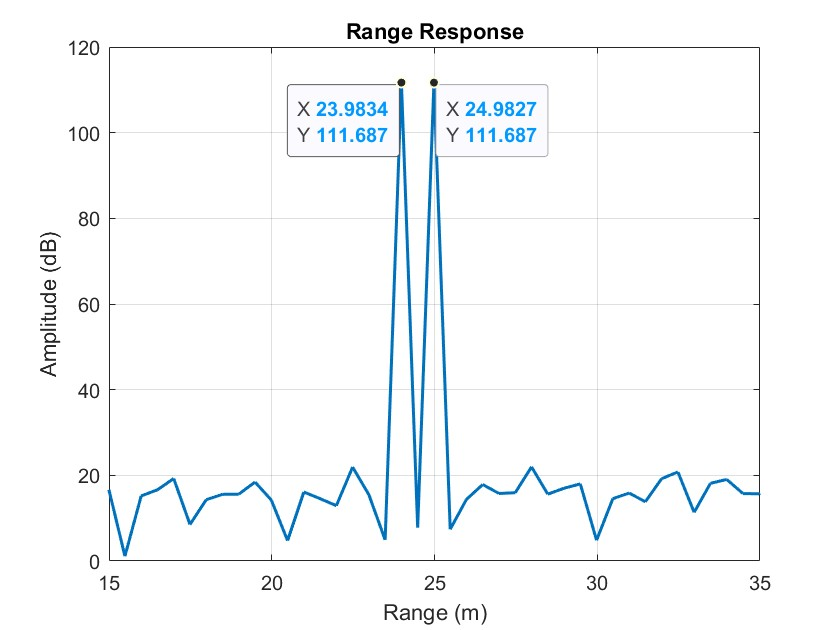
\includegraphics[width=0.8\linewidth]{range_resolution.jpg}}
	    	\caption{Range Response of Two Closely Placed Targets}
	    	\label{fig::range_resolution}
	\end{figure}
		
	Clearly, the minimum range separation at which the radar can distinguish two objects is when the objects are separated by a single range gate. This implies a range resolution of 0.5 m. This is consistent with the theoretical range resolution.
	
	The peak sidelobe ratio (PSLR) is the ratio of the range response peak to its highest sidelobe. The range response of an FMCW radar is the FFT of a tone (i.e. a sinc function). Therefore, the PSLR can vary drastically with the location of the FFT samples. To get a more consistent PSLR measurement, we zero-pad the fast-time FFT. Doing so, results in the following range response:
	
	\begin{figure}[H]
	    	\centering
	    	\fbox{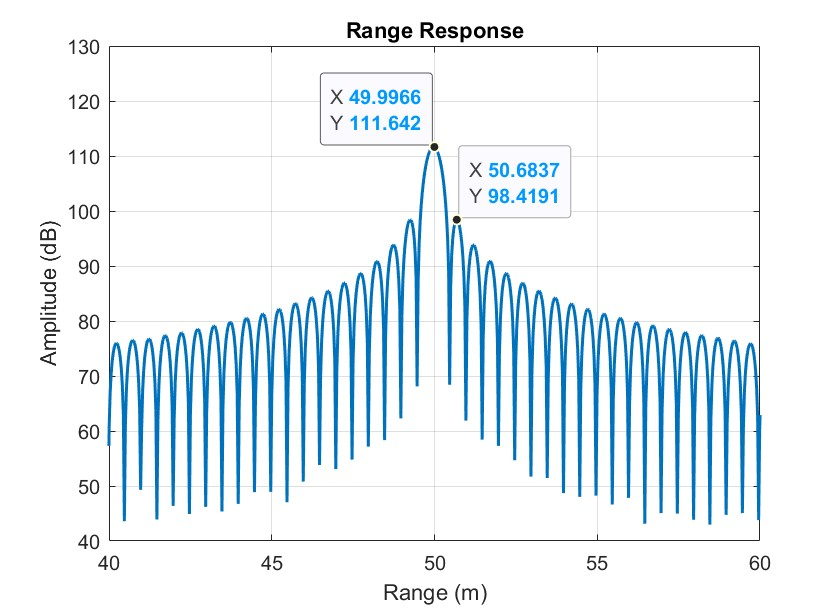
\includegraphics[width=0.8\linewidth]{pslr_no_window_zpad.jpg}}
	    	\caption{PSLR Measurement with Zero Padding in Fast-Time FFT}
	    	\label{fig::pslr_zpad}
	\end{figure}
	
	Examining the figure, we measure a PSLR of 13.27 dB, which is the expected PSLR measurement for a sinc function.
	
	Note that we can improve the PSLR by applying a window. However, this will also degrade the range resolution by increasing the range response's mainlobe width. First, we consider a Chebyshev window with an 80dB peak to sidelobe ratio. The resulting range response is shown in Figure \ref{fig::plsr_window}.
	
	\begin{figure}[H]
	    	\centering
	    	\fbox{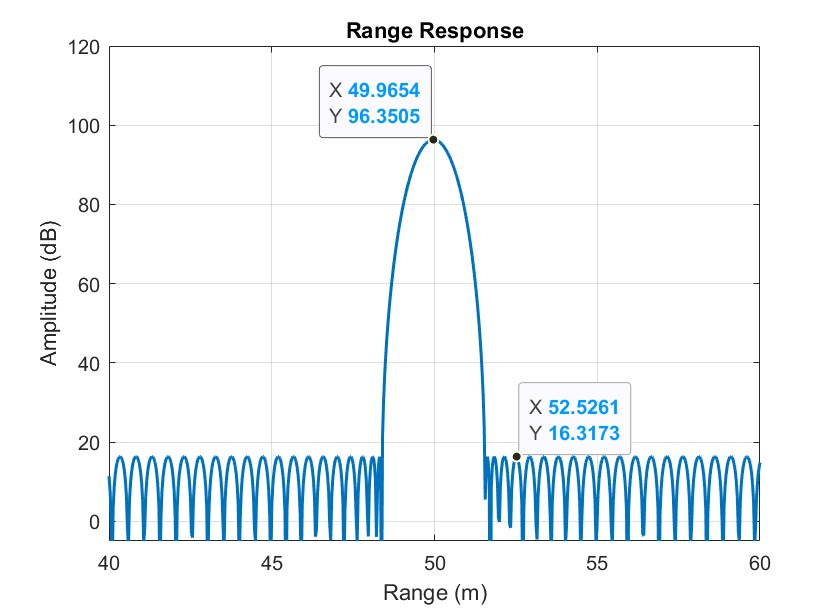
\includegraphics[width=0.8\linewidth]{pslr_with_window.jpg}}
	    	\caption{PSLR Measurement with Chebyshev Window}
	    	\label{fig::plsr_window} 
	\end{figure}
	
	Examining the range response, we achieve the expected PSLR of 80 dB. However, the mainlobe width is also increased by a factor of 3.2, which in term degrades the range resolution by a factor of 3.2. Other windows can be selected, which may off a better trade-off between range resolution and PSLR. Consider a taylor window, for example. It achieves a PSLR of 30.44 dB while only degrading the range resolution by a factor of 1.5.
	
	\begin{figure}[H]
	    	\centering
	    	\fbox{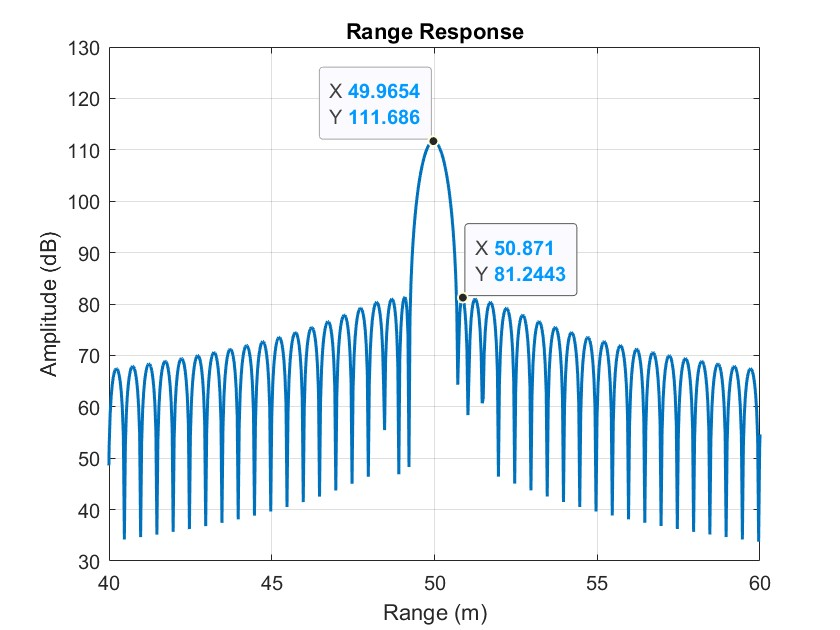
\includegraphics[width=0.8\linewidth]{pslr_with_taylor_window.jpg}}
	    	\caption{PSLR Measurement with Taylor Window}
	    	\label{fig::plsr_taylor_window} 
	\end{figure}
	
	We can measure the doppler tolerance of the system, by examining the PSLR in the presence of uncompensated doppler. In Figure \ref{fig::doppler_tolerance}, we show the PSLR when an 80 dB Chebyshev window is applied while sweeping the uncompensated doppler from $-v_{ua}$ to $v_{ua}$.
	
	\begin{figure}[H]
		\centering
	    	\fbox{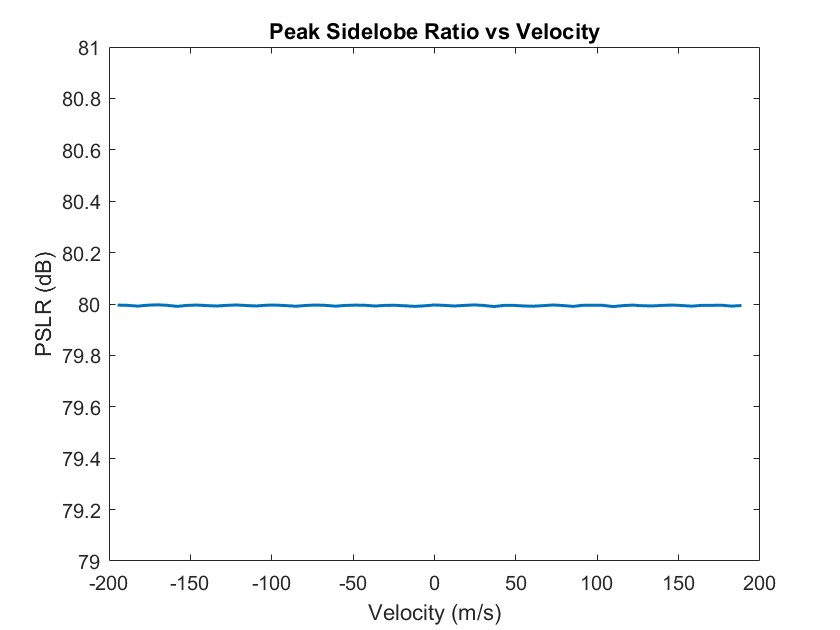
\includegraphics[width=0.8\linewidth]{doppler_tolerance.jpg}}
	    	\caption{PSLR Measurement with Uncompensated Doppler}
	    	\label{fig::doppler_tolerance} 
	\end{figure}
	
	Note that the PSLR is independent of the uncompensated doppler. This is because the uncompensated doppler simply adds to the frequency of the input tone. This can introduce range error through a process known as range-doppler coupling. However, as long as the doppler shift is in the first ambiguity, we can compensate for any introduced range error.
	
	The unambiguous range and velocity of the system can be computed according to Equation (\ref{eq::unambig_range}) and Equation (\ref{eq::unambig_velocity}). This results in the following:
	
	\begin{equation}
		R_{ua} = 750\ \text{m}
	\end{equation}
	
	\begin{equation}
		v_{ua} \approx 194.8\ \text{m/s}
	\end{equation}
	
	We can measure the ambiguous range and velocity by placing a reflecting object at ranges and velocities that exceed these limits. For instance, to measure the unambiguous range, we place an object at a range of 1250 m and examine the resulting range doppler matrix (RDM).
	
	\begin{figure}[H]
	    	\centering
	    	\fbox{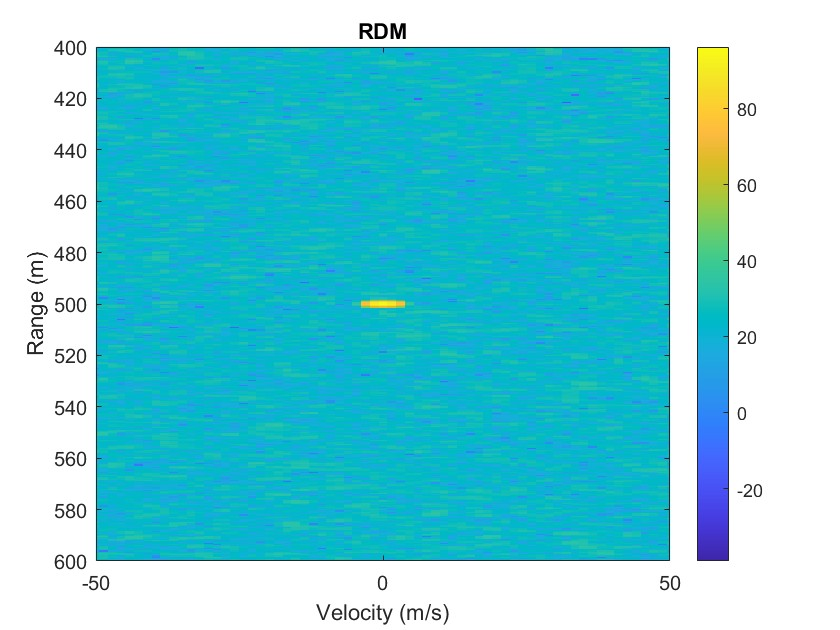
\includegraphics[width=0.8\linewidth]{ambig_range.jpg}}
	    	\caption{Range Doppler Matrix for Object at Ambiguous Range}
	    	\label{fig::ambig_range} 
	\end{figure}
	
	Figure \ref{fig::ambig_range} shows the RDM for this ambiguous range. The radar measures a range of 500.15 m. For an ideal system, the measured range is given as follows:
	
	\begin{equation}
		R_m = R\ \text{mod}\ R_{ua}
	\end{equation}
	
	Our measured range is consistent with this result thereby confirming the theoretical unambiguous range.
	
	We can confirm the unambiguous velocity in a similar manner. To do so, we measure the velocity of an object traveling at 250 m/s.
	
	\begin{figure}[H]
	    	\centering
	    	\fbox{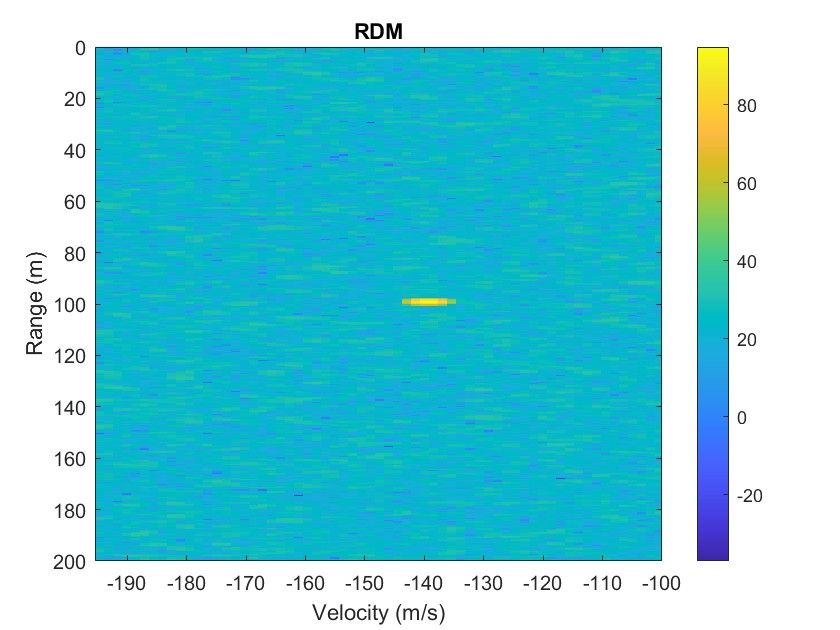
\includegraphics[width=0.8\linewidth]{ambig_velocity.jpg}}
	    	\caption{Range Doppler Matrix for Object at Ambiguous Velocity}
	    	\label{fig::ambig_velocity} 
	\end{figure}
	
	Figure \ref{fig::ambig_velocity} shows the RDM for this ambiguous velocity. The radar measures a velocity of -139.92 m/s. For an ideal system, the measured velocity can be computed as follows:
	
	\begin{equation}
		v_p = v\ \text{mod}\ 2v_{ua}
	\end{equation}
	
	\begin{equation}
		v_m = \begin{cases}
			v_p & 0 \leq v_p < v_{ua} \\
			v_p - 2v_{ua} & v_{ua} \leq v_p < 2v_{ua}
		\end{cases}
	\end{equation}
	
	Our measured velocity is consistent with this result.
	
	According to \cite{richards-2005}, the SNR at the receiver input is given by the following equation:
	
	\begin{equation}
		\chi = \frac{P_tG^2\lambda^2\sigma}{(4\pi)^3R^4kT_0\beta_nF_nL_sL_{\alpha}(R)}
	\end{equation}
	
	Each of the variables in the above expression are defined as follows:
	
	\begin{center}
	\begin{tabular}{|c|c|}
		\hline
		Variable & Definition \\
		\hline
		$P_t$ & Transmit Power \\
		\hline
		$G$ & Antenna Gain \\
		\hline
		$\lambda$ & Wavelength \\
		\hline
		$\sigma$ & RCS \\
		\hline
		$R$ & Distance to Object \\
		\hline
		$k$ & Boltzmann's Constant \\
		\hline
		$T_0$ & Temperature \\
		\hline
		$\beta_n$ & Noise Equivalent Bandwidth \\
		\hline
		$F_n$ & Noise Figure \\
		\hline
		$L_s$ & System Loss \\
		\hline
		$L_{\alpha}(R)$ & Atmospheric Loss \\
		\hline
	\end{tabular}
	\end{center}	
	
	If we consider only the contributions of the transmit power and noise equivalent bandwidth, we can derive the relationship among the remaining variables:
	
	\begin{equation}
		\chi \propto \frac{P_t}{\beta_n}
		\label{eq::snr_propto}
	\end{equation}
	
	Note that the SNR in the RDM is greater than the input SNR by a factor of $G_{sp}$, where $G_{sp}$ is the SNR gain due to signal processing. The signal processing gain for the FMCW radar is given by:
	
	\begin{equation}
		G_{sp} = G_{fast}G_{slow}
	\end{equation}
	
	Here, $G_{fast}$ is the SNR gain due to fast-time processing, and $G_{slow}$ is the SNR gain due to slow-time processing. The fast-time SNR gain is given as follows:
	
	\begin{equation}
		 G_{fast} = \frac{M_{fast}}{L_{fast}} = \frac{f_s/PRF}{L_{fast}}
		 \label{eq::fmcw_fast_time_snr_gain}
	\end{equation}
		
	where $f_s$ is the sample rate and $L_{fast}$ is the SNR loss due to the fast-time FFT window. Using an 80 dB Chebyshev window, we get the following for $G_{fast}$:
	
	\begin{equation}
		G_{fast} \approx 860.8422
	\end{equation}
	
	Similarly, for the slow-time SNR gain, we have
	
	\begin{equation}
		G_{slow} = \frac{M_{slow}}{L_{slow}} = \frac{\#PRI}{L_{slow}}
	\end{equation}
		
	where $L_{slow}$ is the SNR loss due to the slow-time FFT window. Using an 80 dB Chebyshev window, we get the following solution for $G_{slow}$:
	
	\begin{equation}
		G_{slow} \approx 146.4771
	\end{equation}
	
	Therefore, the overall signal processing SNR gain is given by:
	
	\begin{equation}
		G_{sp} \approx 126094
	\end{equation}
	
	Or equivalently,
	
	\begin{equation}
		 {G_{sp}}_{(dB)} \approx 51.0069\ \text{dB}
	\end{equation}
	
	If we input a signal with an SNR of 20 dB and measure the SNR in the RDM, we obtain a value of 70.01 dB, which is consistent with the expected signal processing gain.
		
     \section {Communication (OFDM)}
     
	 \subsection {Background}
	 
	 	In this section, we provide background on OFDM (orthogonal frequency-division multiplexing). OFDM is a form of multicarrier modulation. In multicarrier modulation, the total channel bandwidth is divided into multiple subchannels, so that each subchannel experiences relatively flat fading. The subchannel spacing of OFDM differs from other forms of multicarrier modulation. OFDM modulates symbols on orthogonal subcarriers of the following form:
	 	
	 	\begin{equation}
	 		s_k(t) = e^{j2{\pi}kt/T_s}\text{rect}(t/T_s)
	 	\end{equation}
	 	
	 	where $T_s$ is the symbol duration.
	 	
	 	The orthogonality of the subcarriers allows the bandwidth of neighboring subchannels to be partially overlapped, improving spectral efficiency.
	 	
	 	A block diagram of an OFDM system is given in Figure \ref{fig::ofdm_block_diagram}.
		
	 	\begin{figure}[H]
	    		\centering
	    		\fbox{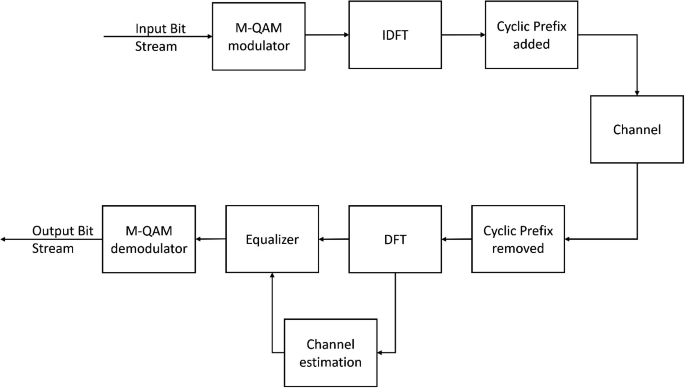
\includegraphics[width=0.9\linewidth]{OFDM Block diagram}}
	    		\caption{OFDM block diagram.\cite {10.1007/978-981-16-2406-3_61}}
	    		\label{fig::ofdm_block_diagram}
		\end{figure}
		
		When a bit stream is received, it is modulated using the desired 2-D modulation scheme PSK, QAM, etc...). Then, it is placed into an FFT bin corresponding to a data subcarrier. Non-data carriers are reserved for pilot and null subcarriers as illustrated in Figure \ref{fig::ofdm_subcarriers}.
		
		\begin{figure}[H]
	    		\centering
	    		\fbox{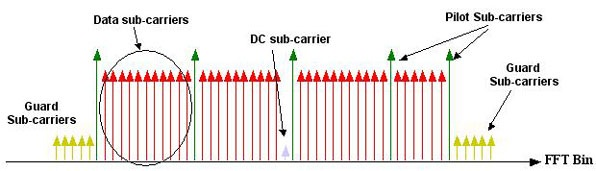
\includegraphics[width=0.9\linewidth]{OFDM subcarriers}}
	    		\caption{OFDM subcarriers. \cite {inproceedings}}
	    		\label{fig::ofdm_subcarriers}
		\end{figure}
		
		Typically, null carriers are placed at the edges of the band to reduce interference between neighboring channels. A null carrier is also typically placed at DC to avoid problems with DC offsets in the D/A and A/D \cite{802_11a_standard}. An IFFT then modulates each of the symbols with its respective subcarrier.
		
		To deal with the effects of multi-path, a cyclic prefix is added to each of the OFDM symbols. The cyclic prefix appends the last L samples of an OFDM symbol to the beginning of the OFDM symbol as illustrated in Figure \ref{fig::cylic_prefix}.
		
		\begin{figure}[H]
	    		\centering
	    		\fbox{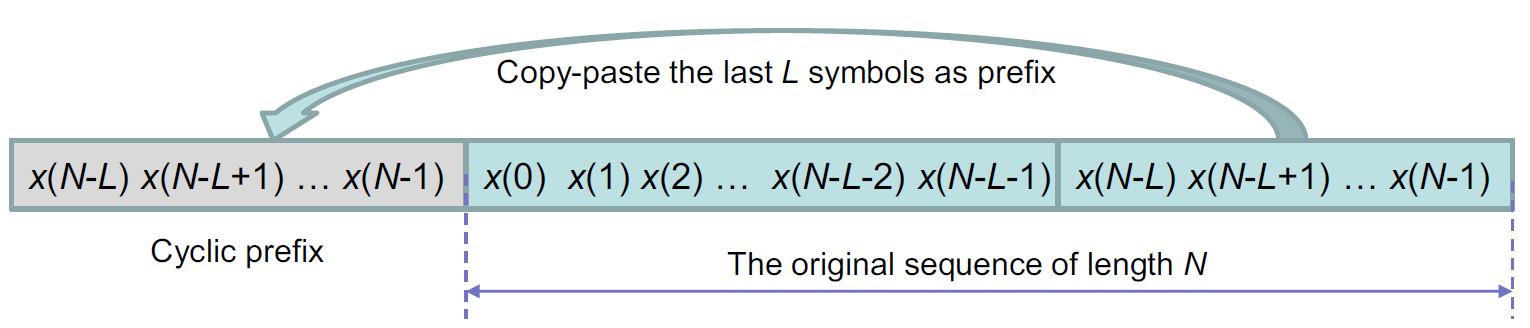
\includegraphics[width=0.9\linewidth]{cyclic_prefix.png}}
	    		\caption{OFDM Cyclic Prefix}
	    		\label{fig::cylic_prefix}
		\end{figure}
		
		At this stage, we can also add a window to reduce the out-of band spectrum. In the case of windowing, the first \newline $L/2 + L_{win}$ samples are appended to the end of the symbol and the last $L/2 + L_{win}$ samples are appended to the beginning of the symbol. This is illustrated in Figure \ref{fig::ofdm_windowing}.
		
		\begin{figure}[H]
	    		\centering
	    		\fbox{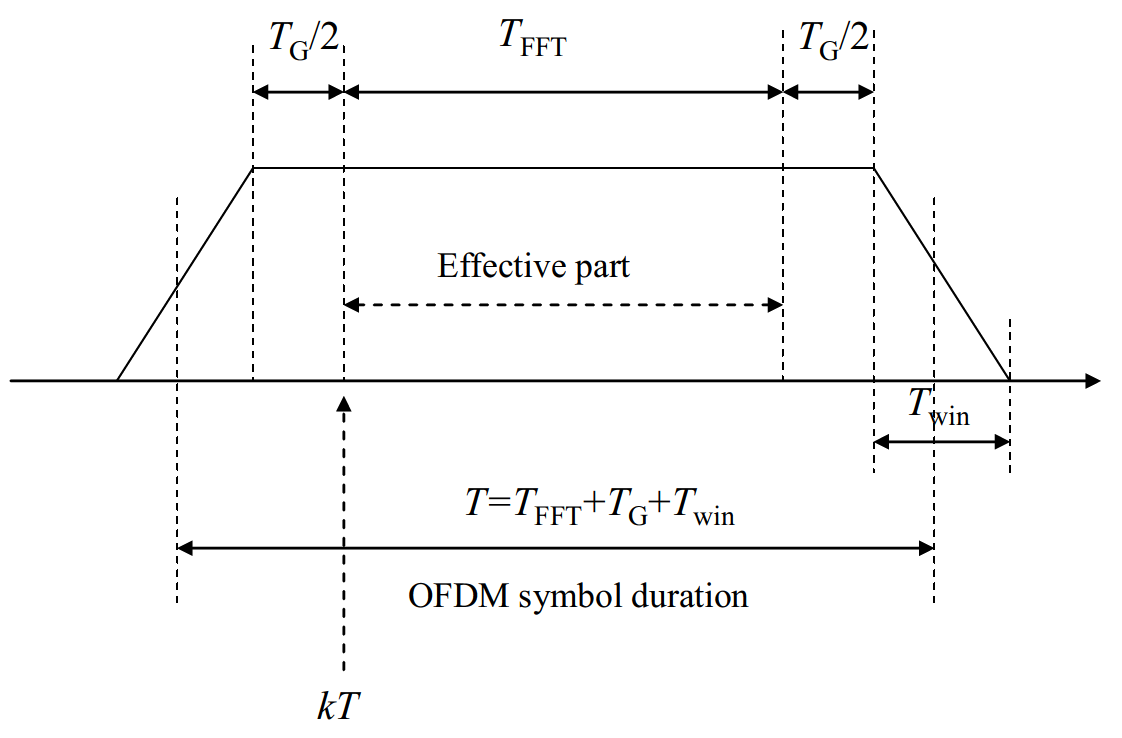
\includegraphics[width=0.9\linewidth]{ofdm_windowing.png}}
	    		\caption{OFDM Symbol with Windowing}
	    		\label{fig::ofdm_windowing}
		\end{figure}
		
		Then a window is multiplied element-wise with the symbol. A commonly applied window is
		
		\begin{equation}
			w_1(t) = \frac{1}{2}[1 - \cos\pi(t + T_{win} + T_G/2)/T_{win}]
		\end{equation}
		
		\begin{equation}
			w_2(t) = \frac{1}{2}[1 - \cos\pi(t - T_{FFT})/T_{win}]
		\end{equation}
		
		\begin{equation}
			w(t) = \begin{cases}
				w_1(t), & T_1 \leq t < T_2 \\
				1.0, & T_2 \leq t < T_3 \\
				w_2(t), & T_3 \leq t < T_4
			\end{cases}
		\end{equation}
		
		where $T_1$, $T_2$, $T_3$, and $T_4$ are defined as follows:
		
		\begin{equation}
			T_1 = -T_{win} - T_G/2
		\end{equation}
		
		\begin{equation}
			T_2 = -T_G/2
		\end{equation}
		
		\begin{equation}
			T_3 = T_{FFT} + T_G/2
		\end{equation}
		
		\begin{equation}
			T_4 = T_{FFT} + T_G/2 + T_{win}
		\end{equation}
		
		At the receiver, the window and or cyclic prefix are removed before the signal is demodulated with an FFT. Because of the cyclic prefix, each of the received multi-path components are a circularly-shifted copies of the transmitted signal. After the FFT, the multi-path components result in a complex weight for each of the FFT bins. We can remove this complex weighting by equalizing the received symbol. To perform equalization, we can estimate estimate the channel at each of the pilot carriers:
		
		\begin{equation}
			\hat{H}_{p_k} = \frac{Y_{p_k}}{X_{p_k}}
		\end{equation}
		
		We then can interpolate the channel estimate to get an estimate of the channel at each of the data carriers. Finally, we can compute equalization weights $A_k$ using either an zero-forcing or MMSE equalizer.
		
		\begin{equation}
			A_{\text{ZF}_k} = \frac{1}{\hat{H}_k}
		\end{equation}
		
		\begin{equation}
			A_{\text{MMSE}_k} = \frac{\hat{H}_k^{*}}{|\hat{H}_k|^2 + 1/SNR}
		\end{equation}
		
		After equalization, we should be obtain to correctly reconstruct the symbols contained in the OFDM data carriers. Each of these symbols can then be demodulated to obtain the received bit stream.
		
		% Look at moving the capacity formulas into result
		
Some of OFDM's perform metrics of interest that we are going to analize in this paper include but are not limited to:

\begin{itemize}
\item Received SNR
\item Bit Error Rate (BER)
\item Channel Capacity
\end{itemize}

One channel's property needs to be analysed and compared is the channel capacity. We use the simple fromula below (Shannon-Hartley theorem) to calculate the channel capacity. 
Where Bk is the bandwidth of the k-th subcarrier, Pk, transmit power, Hk, frequency response magnitude and Nk is a noise power.   
%Where H (m, n) , Hmn is the channel frequency response of the n symbol on the m sub carrier. 
	
		%\begin{equation}
		%	    		C_{m,n} = \text{log}_2\left(1 + \text{SNR}|H(m,n)|^2\right)
	    	%	\label{eq:ofdm_capacity}
		%\end{equation}

			\begin{equation}
			C_{k} = B_{k}.\text{log}_2\left(1 +\frac{ \text P_{k}.|H_{k}|^2}{N_{k}}\right)
	    		\label{eq:ofdm_capacity}
	    		\end{equation}

\subsection {Simulation and Performance}
      
      We have developed comprehensive MATLAB code to evaluate the performance of an OFDM communication system. Metrics of interest include the peak to average power ratio (PAPR), the bit error rate (BER) in an AWGN channel, the BER in presence of Rayleigh fading, and the capacity of the system.
      
      For this analysis, we chose to evaluate an OFDM 802.11p system because the 802.11p standard is applicable to VNV communication \cite{802_11p_abdelgader}. The 802.11p standard operates in the DRC Band (5.850 GHz to 5.925 GHz) and uses 64 subcarriers sampled at a rate of 10 MHz. A 16 sample cyclic prefix is added, increasing the symbol duration from 6.4 ${\mu}s$ to 8.0 ${\mu}s$. Of the 64 subcarriers, 48 are data carriers, and 4 are pilots. Pilots are specifically located at $\{-21, -7, 7, 21\}$. Data carriers cover all the remaining carriers in range $[-26, 26]$ except the DC subcarrier, which is a null carrier.
      
    The power spectral density of the transmitted OFDM signal is shown in Figure \ref{fig::ofdm_psd}.
    
    \begin{figure}[H]
    		\centering
    		\fbox{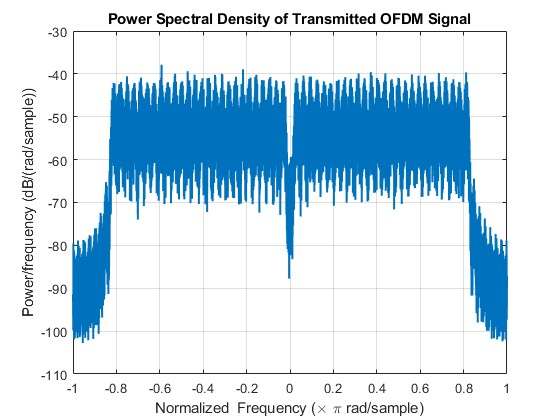
\includegraphics[width=0.8\linewidth]{OFDM Power spectral density}}
    		\caption{OFDM Power Spectral Density}
    		\label{fig::ofdm_psd}
	\end{figure}
    
    The location of null carrier is also consistent with the 802.11p standard. We were able to perform power measurements on this signal to determine the PAPR. When the data carriers are modulated using QPSK modulation, we measure a PAPR of 11.8 dB. The measured PAPR is significant because it forces us to run the high power amplifier at reduced power levels, which can degrade the transmitted power and in turn the SNR of the system.
    
    To evaluate the BER in an AWGN channel, we add gaussian noise to the transmitted signal to achieve a given SNR. Then, we process the resulting signal with a model of the OFDM receiver. After FFT processing, we can generate a constellation diagram from the resulting data carriers. Figure \ref{fig::rx_constellation_diagram} shows the received constellation diagram for an OFDM signal using QPSK modulation at 20 dB SNR.
      
      \begin{figure}[H]
		\centering
    		\fbox{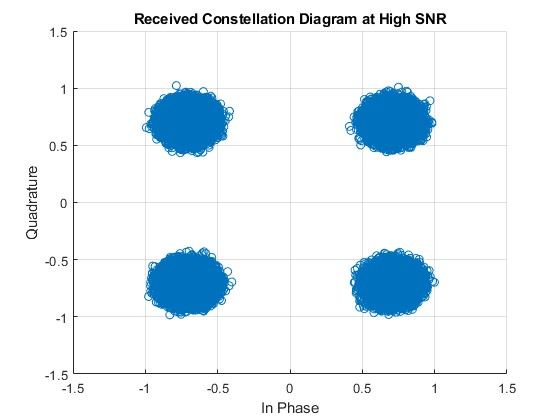
\includegraphics[width=0.8\linewidth]{OFDM AWGN Constellation}}
    		\caption{OFDM Received Constellation after AWGN Channel}
    		\label{fig::rx_constellation_diagram}
  	  \end{figure}
    
    		The expected bit error rate (BER) for a single OFDM subcarrier is identical to the BER of a single carrier system, when the SNR of the given subcarrier is considered. For QPSK, this is approximately given by
		
		\begin{equation}
			P_b(\rho_b) \approx Q(\sqrt{2\rho_b})
		\end{equation}
		
		where $\rho_b$ is the SNR per bit. If the modulation is the same for each OFDM subcarrier, the BER is the mean BER for all active data carriers. In Figure \ref{fig::ofdm_awgn_ber}, we examine the BER of an OFDM system vs SNR.
		
		\begin{figure}[H]
			\centering
    			\fbox{\includegraphics[width=0.8\linewidth]{OFDM AWGN BER vs SNR}}
    			\caption{OFDM BER vs. SNR in AWGN channel}
    			\label{fig::ofdm_awgn_ber}
		\end{figure}
		
		The SNR of each active subcarrier is 64/52 times (or 0.9018 dB) greater that of the received signal because all the signal energy is concentrated in the active subcarriers. After accounting for this SNR gain, the resulting BER is equivalent to the expected BER. 
        
        We also examine the BER of the OFDM receiver in the presence of Rayleigh fading. To do so, we apply Rayleigh fading to the signal amplitude prior to applying additive white gaussian noise. We can then generate a received constellation map for each of the symbols modulated on the data carriers. For 20 dB SNR, the received constellation map is shown in Figure \ref{fig::ofdm_rayleigh_fading}.
        
      \begin{figure}[H]
		\centering
    		\fbox{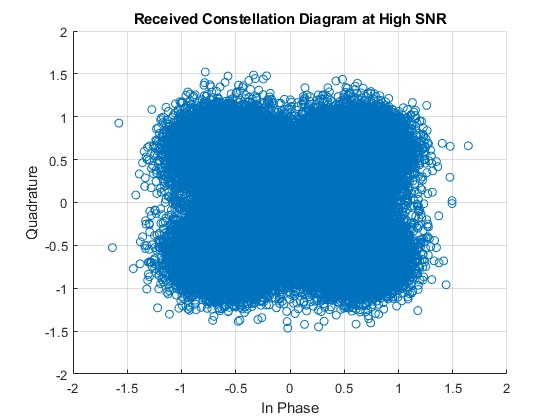
\includegraphics[width=0.8\linewidth]{OFDM Constellation Diagram}}
    		\caption{OFDM Received Constellation Diagram after Rayleigh Fading}
    		\label{fig::ofdm_rayleigh_fading}
  	  \end{figure}
    
    		We can compare the received constellation to the one shown in Figure \ref{fig::rx_constellation_diagram}. Doing so, we observe that the clusters are not easily separable like they were previously, indicating a much higher BER. The average BER in the presence of fading can be computed as follows:
    		
    		\begin{equation}
    			\bar{P}_b = \int_{0}^{\infty}{P_b(\rho)f(\rho)d\rho}
    		\end{equation}
    		
    		$f(\rho)$ is the distribution of the SNR due to Rayleigh fading and is given by
    		
    		\begin{equation}
    			f(\rho) = \frac{1}{\bar{\rho}}e^{-\frac{\rho}{\bar{\rho}}}
    		\end{equation}
    			
    		where $\bar{\rho}$ is the average SNR. In Figure \ref{fig::ofdm_fading_ber}, the measured BER in the presence of Rayleigh fading is compared to the expected BER.
    		
    		\begin{figure}[H]
			\centering
    			\fbox{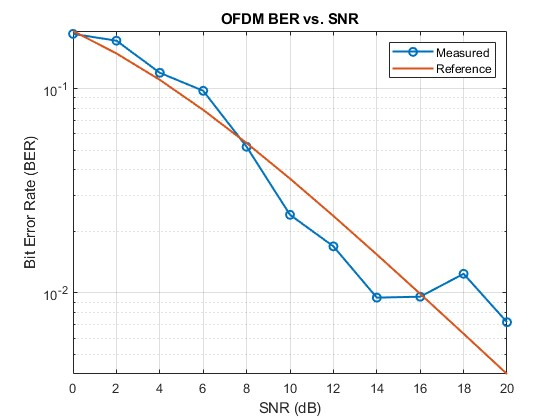
\includegraphics[width=0.8\linewidth]{OFDM BER vs SNR}}
    			\caption{OFDM BER vs. SNR in Rayleigh Fading}
    			\label{fig::ofdm_fading_ber}
  	  	\end{figure}
  	  
  	  	Referring to the figure, the measured BER rate is consistent with the expected BER.
    		
    	  % Look at refactoring this section
    	    	  
  	  For the given parameter, B total=10 MHz, N subcarriers=64, N data=48, P total =1 W (assumed for simplicity) and No=1 nW/Hz, the total channels capacity for given OFDM  with AWGN is around 99.74 Mbps. \par
  	 It is important to highlight the cyclic prefix reduces the effective data rate, which slightly decreases the channel capacity. Adjust for this overhead if needed.
    
    \section {JRC}
		\subsection {Background}

		In this section, we design a JRC system using zero forcing to generate RDMs from OFDM returns. The ideal range response is given by:
		
		\begin{equation}
			x[n] = \delta[n]
		\end{equation}
		
		The frequency response of the ideal range response is flat:
		
		\begin{equation}
			X[k] = 1\ \forall\ 0 \leq k < N 
		\end{equation}
		
		We can generate the ideal range response from any known sequence $z[n]$, which has a non-zero frequency response $Z[k]\ \forall\ 0 \leq k < N$. To generate the ideal range response we can multiply $Z[k]$ element-wise with $H[k]$, where $H[k]$ is defined as follows:
		
		\begin{equation}
			H[k] = \frac{1}{Z[k]} \forall\ 0 \leq k < N
		\end{equation}
		
		After element-wise multiplication, the result is $X[k]$. Finally, we can apply an IFFT to $X[k]$ to generate $x[n]$, the ideal range response.
		
		If we instead receive a circularly-shifted copy of $z[n]$ (i.e. $y[n] = z[[n-m]_N]$), the FFT of the resulting sequence is given as follows:
		
		\begin{equation}
			Y[k] = Z[k]W_N^{km}
		\end{equation}
		
		If we multiply $H[k]$ element-wise with $Y[k]$, we obtain $W_N^{km}$, which results in a range response of $\delta[n-m]$ after IFFT processing. This is the desired result.
		
		In an OFDM system, the reflections will be a circularly shifted copy of the transmitted waveform as long as their delay does not exceed the cyclic prefix. To physically implement this system, we need to consider the last $N$ samples of each transmitted OFDM symbol as $z[n]$.
		
		\begin{figure}[H]
			\centering
    			\fbox{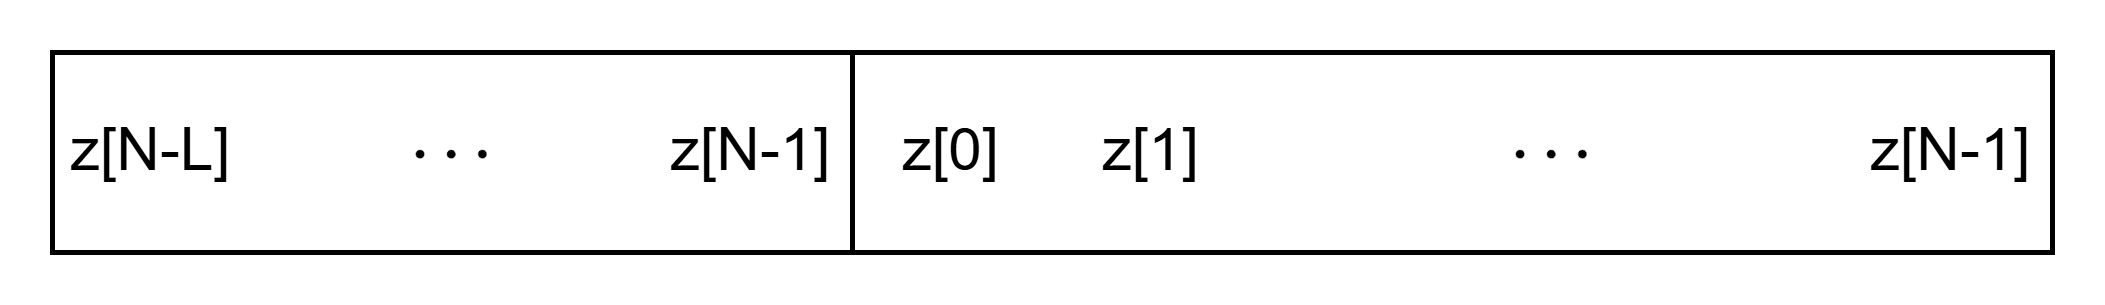
\includegraphics[width=0.8\linewidth]{ofdm_radar_waveform.png}}
    			\caption{OFDM Sample Designation}
    			\label{fig::ofdm_radar_waveform}
  	  	\end{figure}
		
		After transmitting, we can wait $L$ samples before receiving. If the signal has no delay, our range response will be a delta function. However, if the delay of the signal ($m$) is in range $[1, L]$, we will receive a circular-shifted copy of the $z[n]$, and the range response will be a delayed delta function of the form $\delta[n-m]$. 
		
		We don't have to take an FFT of $z[n]$ to obtain $Z[k]$. Instead, we can get $Z[k]$ from the OFDM subcarriers prior to IFFT processing. If the cyclic prefix is placed at the start of the symbol as shown in Figure \ref{fig::cylic_prefix}, $Z[k]$ is identical to the IFFT input. If the window is divided evenly between the start and the back of symbol as shown in Figure \ref{fig::ofdm_windowing}, $Z[k]$ is the IFFT input multiplied elementwise with $W_N^{kL/2}$.
		
		In the 802.11p standard, not all of the subcarriers are non-zero, which prevents us from fully realizing this system. However, we can instead invert all of the non-zero subcarriers, when determining the FFT of our matched filter, $H[k]$. The resulting frequency response is shown in Figure \ref{fig::ofdm_radar_freq_resp_no_window}.
		
		\begin{figure}[H]
			\centering
    			\fbox{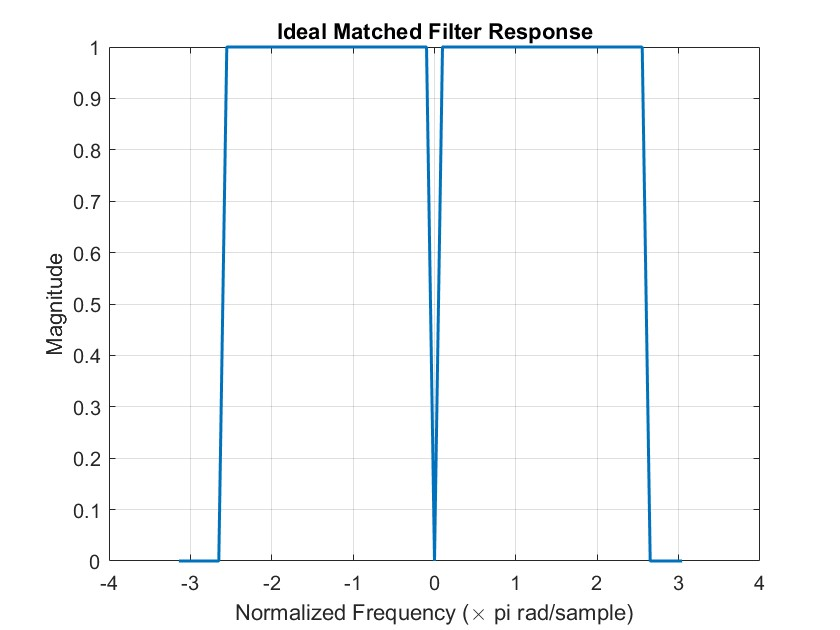
\includegraphics[width=0.8\linewidth]{ideal_frequency_response_no_window.jpg}}
    			\caption{Ideal Frequency Response with Zero Subcarriers}
    			\label{fig::ofdm_radar_freq_resp_no_window}
  	  	\end{figure}
		
		We can take an IFFT to determine the resulting range response. However, because the frequency response is no longer flat, we will not be left with a delta function. Instead we expect a sinc function minus a DC offset due to the missing DC subcarrier. The corresponding range response is shown in Figure \ref{fig::ofdm_radar_range_resp_no_window}.
		
		\begin{figure}[H]
			\centering
    			\fbox{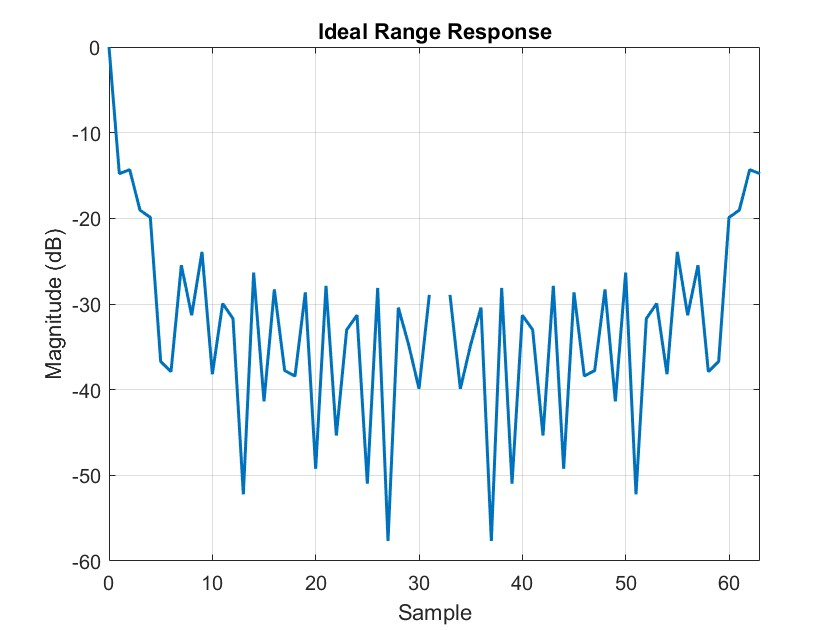
\includegraphics[width=0.8\linewidth]{ideal_range_response_no_window.jpg}}
    			\caption{Ideal Range Response with Zero Subcarriers}
    			\label{fig::ofdm_radar_range_resp_no_window}
  	  	\end{figure}
		
		The sinc-like appearance of the range response is not readily apparent. However, we can zero-pad the IFFT to increase the resolution of the range response. We must perform this zero padding in the middle of the input sequence to preserve the relative positions of the non-zero subcarriers.
		
		\begin{figure}[H]
			\centering
    			\fbox{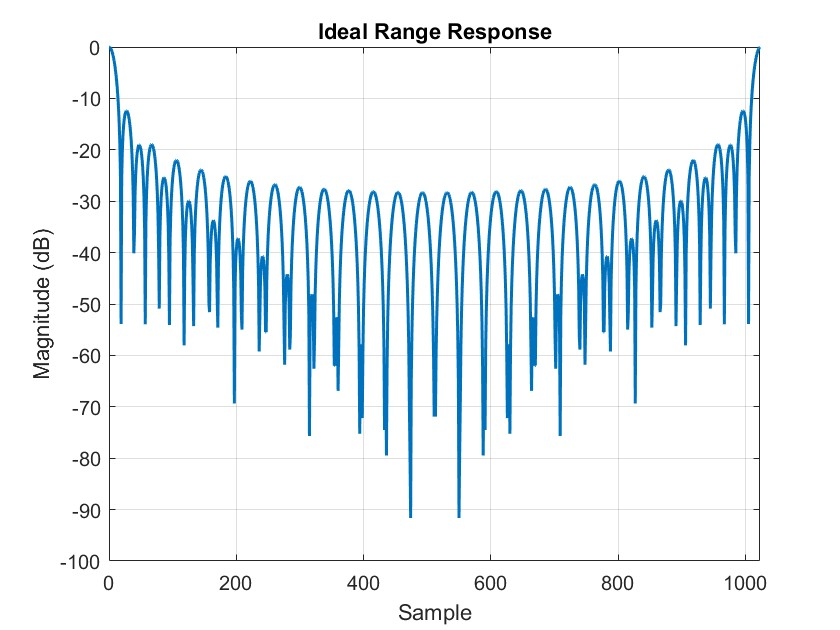
\includegraphics[width=0.8\linewidth]{ideal_range_response_no_window_zpad.jpg}}
    			\caption{Interpolated Range Response with Zero Subcarriers}
    			\label{fig::ofdm_radar_range_resp_no_window_zpad}
  	  	\end{figure}
  	  	
  	  	As was the case with the FMCW radar, we can reduce the sidelobe level with windowing. However, the windowing is now applied in the frequency domain prior to the IFFT. Figure \ref{fig::ofdm_radar_freq_resp_with_window} shows the frequency response after a 80 dB Chebyshev window is applied.
  	  	
  	  	\begin{figure}[H]
			\centering
    			\fbox{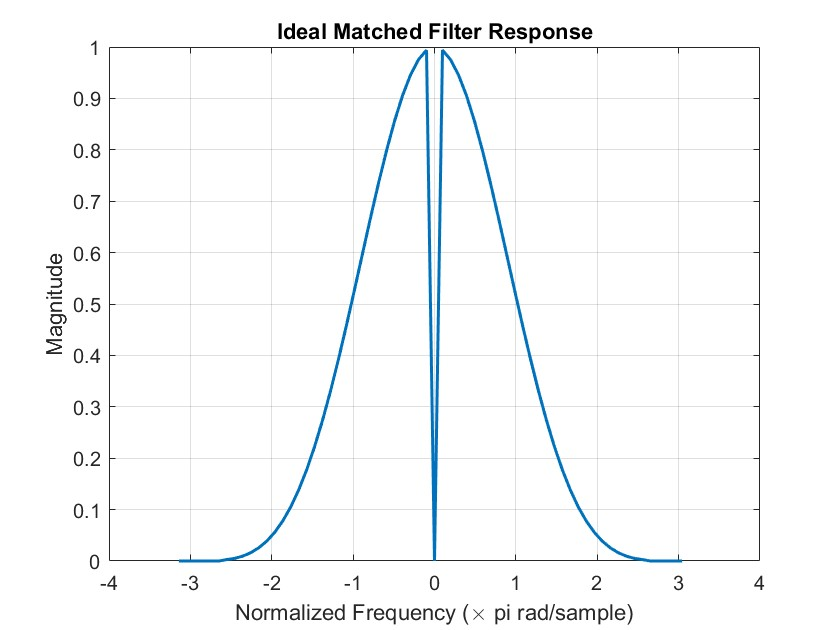
\includegraphics[width=0.8\linewidth]{ideal_freq_response_with_window.jpg}}
    			\caption{Ideal Frequency Response after Windowing}
    			\label{fig::ofdm_radar_freq_resp_with_window}
  	  	\end{figure}
  	  	 
  	  	The corresponding range response is shown in Figure \ref{fig::ofdm_radar_range_resp_with_window}.
  	  	
  	  	\begin{figure}[H]
  	  		\centering
    			\fbox{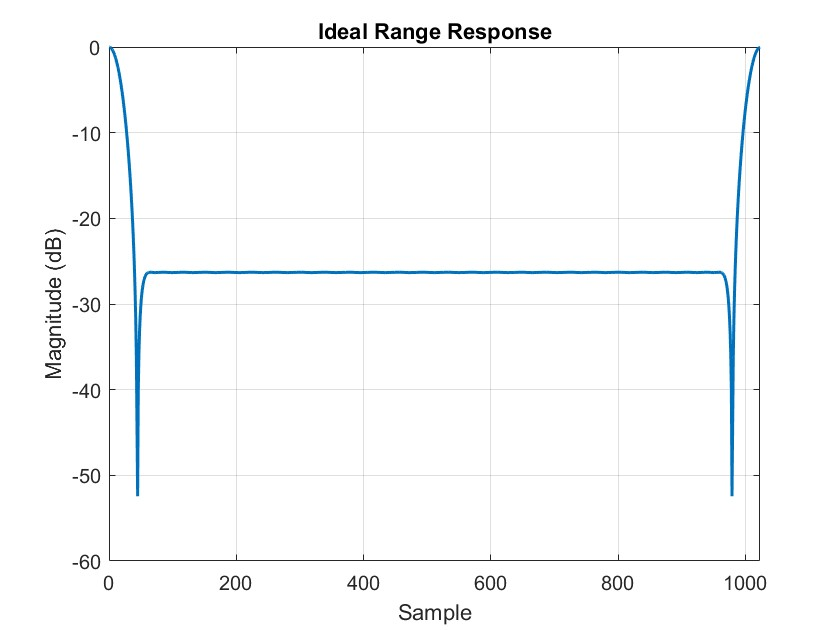
\includegraphics[width=0.8\linewidth]{ideal_range_response_with_window_zpad.jpg}}
    			\caption{Ideal Range Response after Windowing}
    			\label{fig::ofdm_radar_range_resp_with_window}
  	  	\end{figure}
  	  	
  	  	Note that the missing DC subcarrier severely limits the peak to sidelobe performance. As previously mentioned, the DC subcarrier has been nulled to avoid problems with DC offsets in the D/A and the A/D. It is possible to re-add the DC carrier. However, the OFDM receiver may need more complex IF sampling to take advantage it. As an alternative the transmitter can use the DC subcarrier and the OFDM receiver can ignore it. Note that this will degrade the capacity due to less available power for the other subcarriers. The range response with an 80 dB Chebyshev window after adding a DC subcarrier is shown in Figure \ref{fig::ofdm_radar_range_resp_with_zero_subcarrier}.
  	  	
  	  	\begin{figure}[H]
  	  		\centering
    			\fbox{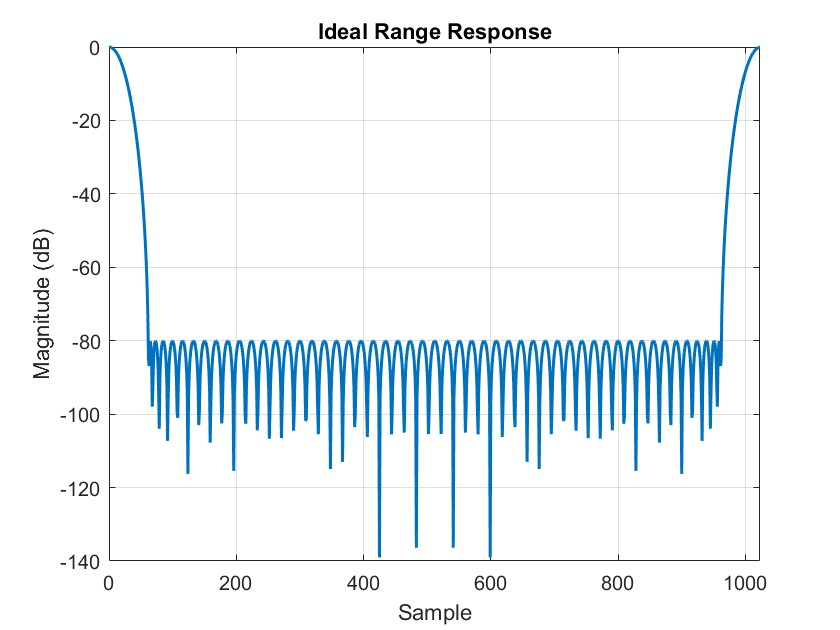
\includegraphics[width=0.8\linewidth]{ideal_range_response_with_zero_subcarrier.jpg}}
    			\caption{Ideal Range Response with Added DC Subcarrier}
    			\label{fig::ofdm_radar_range_resp_with_zero_subcarrier}
  	  	\end{figure}
  	  	
  	  	Note that the range response is now comparable to an FMCW radar. Similar to an FMCW radar, we can stack up many symbols and perform a Doppler FFT across them, to determine the object's velocity. A block diagram of the resulting receiver is shown in Figure \ref{fig::ofdm_radar_receiver}.
  	  	
  	  	\begin{figure}[H]
  	  		\centering
    			\fbox{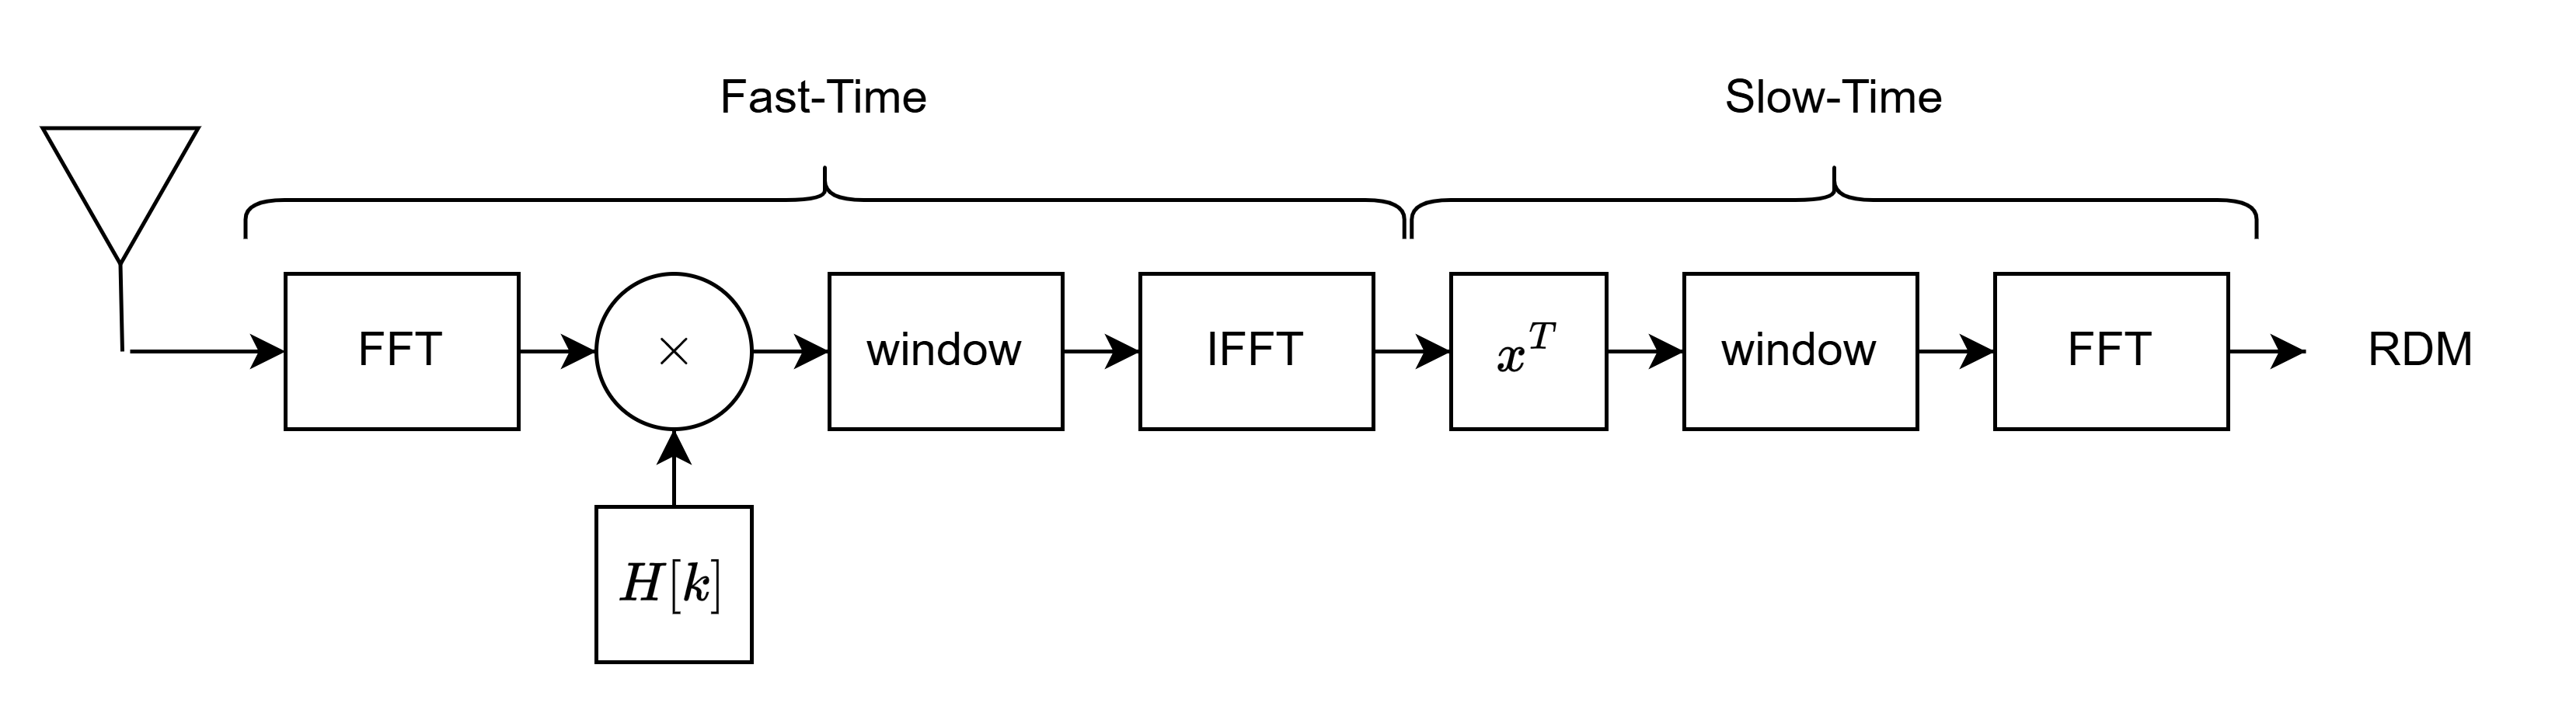
\includegraphics[width=0.9\linewidth]{ofdm_radar_receiver.png}}
    			\caption{OFDM Radar Receiver}
    			\label{fig::ofdm_radar_receiver}
  	  	\end{figure}
  	  	
  	  	The unambiguous range and velocity of the system are given by Equation (\ref{eq::unambig_range}) and Equation (\ref{eq::unambig_velocity}), where the PRF is defined as follows:
  	  	
  	  	\begin{equation}
  	  		PRF = \frac{f_s}{N + L}
  	  	\end{equation}
  	  	
  	  	where $f_s$ is the sample rate, $N$ is the number of subcarriers, and $L$ is the cyclic prefix length.
  	  	
% See if this can be incorporated in introduction	
\iffalse 
 The convergence of radar and communication systems, often referred to as joint radar-communication (JRC), has emerged due to several technological and practical motivations. Some of the primary reasons why radar and communication systems are being integrated listed below :
 
 \begin{itemize}
 \item Spectrum Sharing adn Efficiency (coexisting within the same frequency band)
\item Shared Hardware
\item Autonomous Vehicles
\item Energy Efficiency		 
\end{itemize}		 
		 
The orthogonality or low correlation of the frequency domain allows the two subsystems not to interfere with each other. The disadvantage is that the spectrumutilization of the system is low and energy sharing is difficult to achieve. Other crutial disadvantage we need to overcome is OFDM signals are sensitive to the Doppler shift and multipath effects, which leads to a loss of subcarrier orthogonality and intersymbol interference (ISI) \cite{9992221}.
\fi

\subsection {Simulation and Performance}
      
There are many variables and parameters that can influence the performance of a JRC system. To investigate the performance, we have simulated and compared the results for many scenarios. The first simulation we performed used an OFDM 802.11p transmitter with an OFDM radar receiver. The transmitter includes a null subcarrier at DC which limits the PSLR as shown in Figure \ref{fig::pslr_802_11p_ofdm_radar}.

\begin{figure}[H]
\centering
\fbox{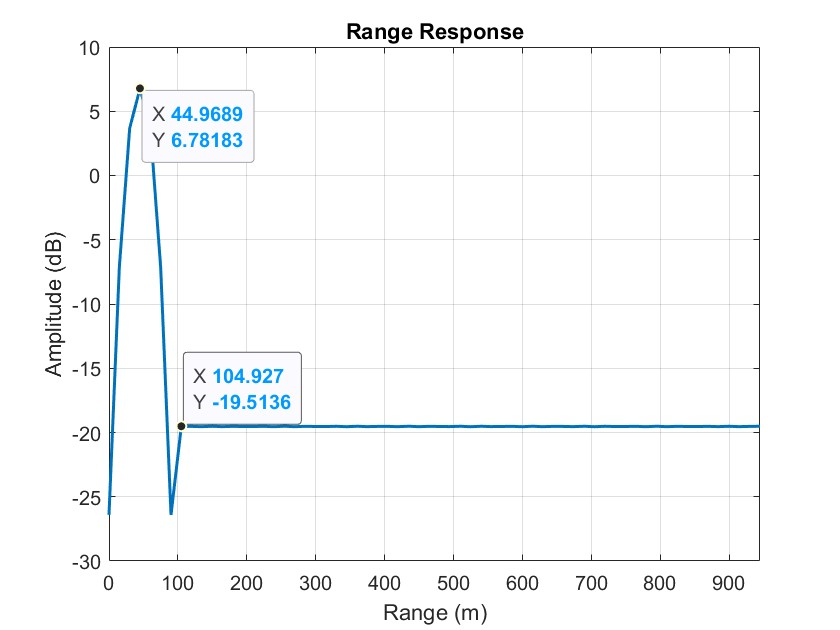
\includegraphics[width=0.8\linewidth]{802_11p_ofdm_range_response.jpg}}
\caption{PSLR Measurement for 802.11p OFDM Radar}
\label{fig::pslr_802_11p_ofdm_radar}
\end{figure}

There we measure a PSLR of 26.30 dB - even when using a 80 dB Chebyshev window. If we add a DC subcarrier to the OFDM transmission as previously suggest, we can achieve a much better PSLR as shown in Figure \ref{fig::pslr_802_11p_mod_ofdm_radar}.

\begin{figure}[H]
\centering
\fbox{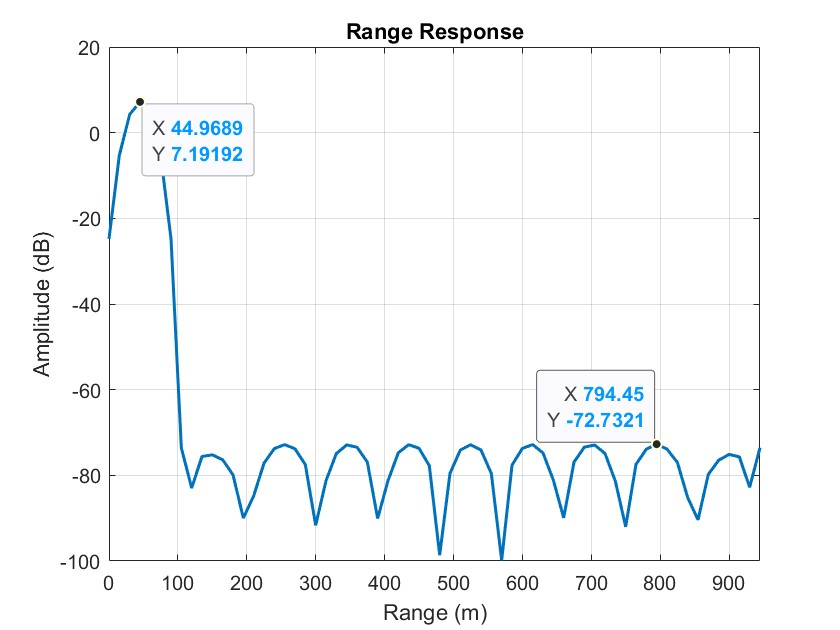
\includegraphics[width=0.8\linewidth]{802_11p_ofdm_mod_range_response.jpg}}
\caption{PSLR Measurement for Modified 802.11p OFDM Radar}
\label{fig::pslr_802_11p_mod_ofdm_radar}
\end{figure}

The PSLR is now 79.92 dB, which is consistent with our 80 dB Chebyshev window. If the receiver can utilize the DC subcarrier, we expect no capacity degradation for the communication system. However, if the DC subcarrier is unused by the receiver, we will see a degradation in capacity.

\iffalse
The capacity of an OFDM system is given by:

\begin{equation}
	C = \text{max}{\sum_{P_j: \sum_j{P_j \leq P}}{W\text{log}_2\left\right)}
\end{equation}
\fi

We can also examine the doppler tolerance of the system by measuring the PLSR while varying the amount of uncompensated doppler shift. The doppler tolerance of the system is shown in Figure \ref{fig::ofdm_radar_doppler_tolerance}.

\begin{figure}[H]
\centering
\fbox{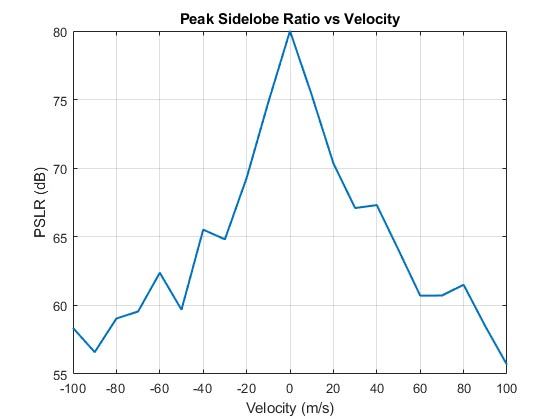
\includegraphics[width=0.8\linewidth]{OFDMRadar_PSLR vs Velocity}}
\caption{OFDM Radar Doppler Tolerance}
\label{fig::ofdm_radar_doppler_tolerance}
\end{figure}

Note unlike the FMCW radar, the PSLR varies with uncompensated doppler. When an 80 dB Chebyshev window is applied, we see a PSLR degradation of ~25 dB for objects with a relative velocity 100 m/s. The PSLR degrades with velocity, because uncompensated doppler creates a mismatch between the FFT of the matched filter $H[k]$ and the FFT of the data $X[k]$.

The JRC system is also only designed to detect returns with delays equal to or smaller than the length of a cyclic prefix. For the 802.11p standard, this range is defined as follows:

\begin{equation}
R_{max} = \frac{ct_0}{2} = \frac{c(L/f_s)}{2} = 240 m
\end{equation}

In Figure \ref{fig::ofdm_radar_pslr_vs_range}, we examine the PSLR against range.

\begin{figure}[H]
\centering
\fbox{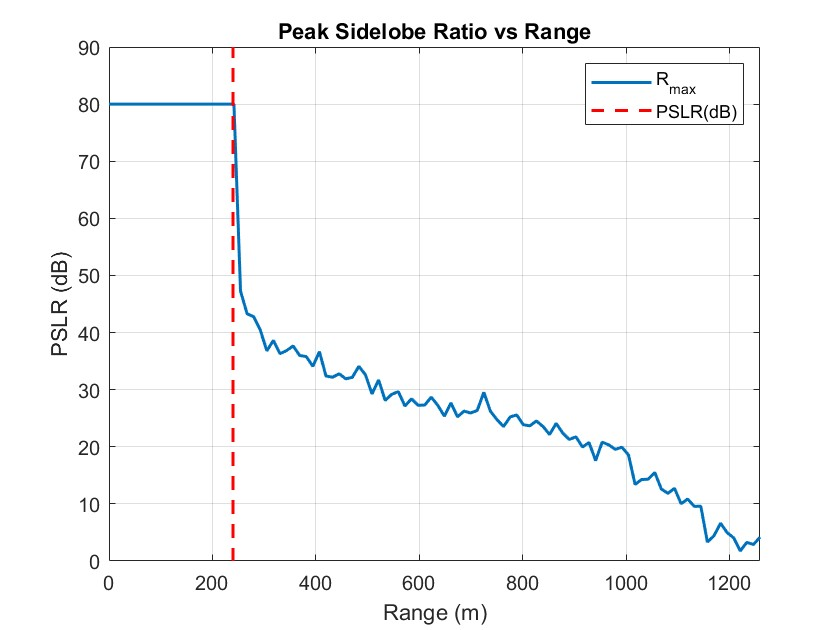
\includegraphics[width=0.8\linewidth]{OFDMRadar_PSLR vs Range}}
\caption{OFDM Radar PSLR vs Range}
\label{fig::ofdm_radar_pslr_vs_range}
\end{figure}

As expected, we see that the PSLR steeply degrades when the range exceeds $R_{max}$.

For an OFDM radar, we have already stated the unambiguous range and velocity. However, due to the demonstrated performance degradations at large ranges and velocities, it is not meaningful to evaluate performance outside of the first range and velocity ambiguity. Even though it is limited to the first ambiguities, an automotive 802.11p radar will still be able to measure an acceptable range of ranges and velocities.

After adding a non-zero DC subcarrier, we can also examine the range resolution of the system. The range resolution is the minimum separation at which two objects are resolvable. For this experiment, we disable the range window to get the finest possible range resolution and zero-pad the IFFT to increase our visibility of the resulting range response. In Figure \ref{fig::ofdm_radar_range_resolution}, we show the range response of two objects separated by 30 m.

\begin{figure}[H]
\centering
\fbox{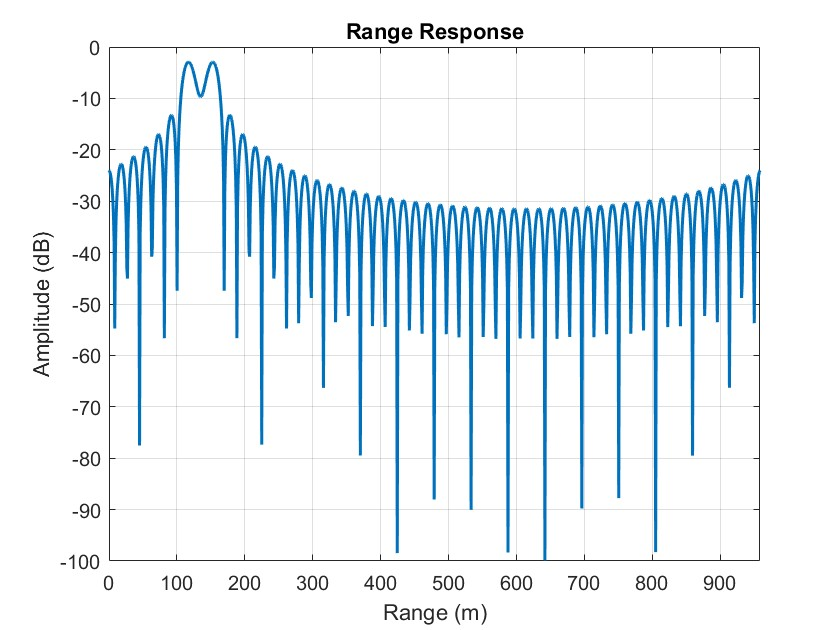
\includegraphics[width=0.8\linewidth]{802_11p_ofdm_range_resolution.jpg}}
\caption{802.11p OFDM Radar Range Resolution Measurement}
\label{fig::ofdm_radar_range_resolution}
\end{figure}

Examining the figure, we can infer that the object separation is approaching the radar's range resolution. For a sinc response, two objects are separated by the range resolution when one response reaches its peak, while the other experiences its first null. In other words the range resolution is half the range response's mainlobe width. In Figure \ref{fig::ofdm_radar_mainlobe_width}, we measure the mainlobe width of the range response without a window function.

\begin{figure}[H]
\centering
\fbox{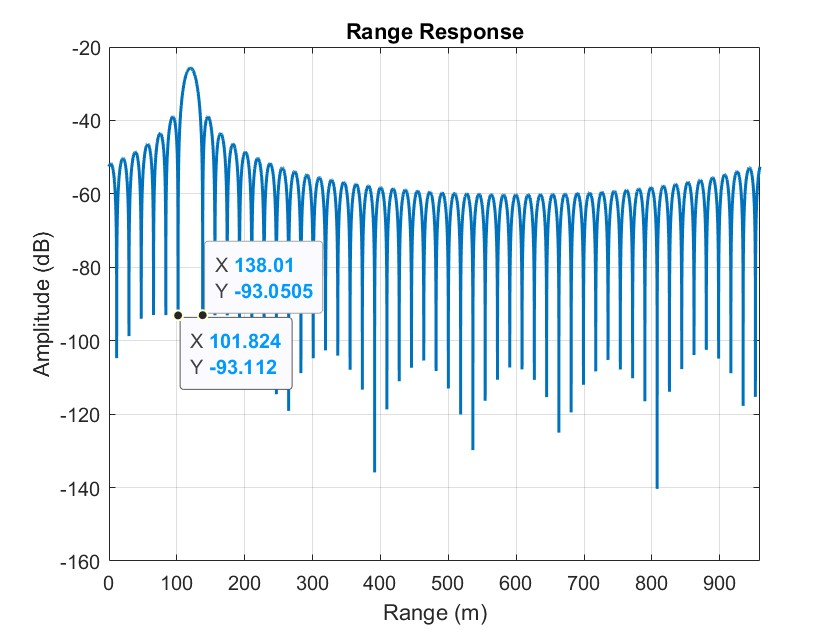
\includegraphics[width=0.8\linewidth]{802_11p_ofdm_range_response_mainlobe_width.jpg}}
\caption{802.11p OFDM Radar Range Response Mainlobe Width}
\label{fig::ofdm_radar_mainlobe_width}
\end{figure}

Examining the above figure, we find that the mainlobe width is $138.01\ \text{m} - 101.824\ \text{m} = 36.186\ \text{m}$. Our measured range resolution is then $36.186\ \text{m} /2 = 18.093 \ \text{m}$. We can also compute the range resolution of the system using Equation (\ref{eq::range_resolution}) with a bandwidth $\beta = 53/64 \times 10\ \text{MHz} = 8.281\ \text{MHz}$. This results in a range resolution of $18.1\ \text{m}$, which is consistent with the measured data.

Note that this range resolution is insufficient for automotive radar applications. However, we can design an OFDM system with more bandwidth in the 77 GHz band that will achieve better range resolution. 

For this system, we increase the bandwidth from 10MHz to 300MHz and scale the OFDM parameters by 16. The updated parameters are included in the table below:

\begin{center}
\begin{tabular}{|c|c|}
\hline
\textbf {Parameter} & \textbf {Value }\\
\hline
Carrier Frequency & 77 GHz \\
\hline
Sample Rate & 300 MHz \\
\hline
Number of Subcarriers & 16x64\\
\hline
Number of Data Carriers & 16x48 + 1 \\
\hline 
Number of Pilot Carriers & 16x4 \\
\hline 
\end{tabular}
\end{center}

With the updated parameters, the active carriers will have a bandwidth of $300 \text{MHz} \times (52 \times 16 + 1)/(64 \times 16) \approx 244\ \text{MHz}$. This bandwidth should correspond to a range resolution of 0.6142 m. In Figure \ref{fig::802_11p_ofdm_improved_range_response_mainlobe_width}, we measure the mainlobe width of the range response to confirm the updated range resolution.


\begin{figure}[H]
\centering
\fbox{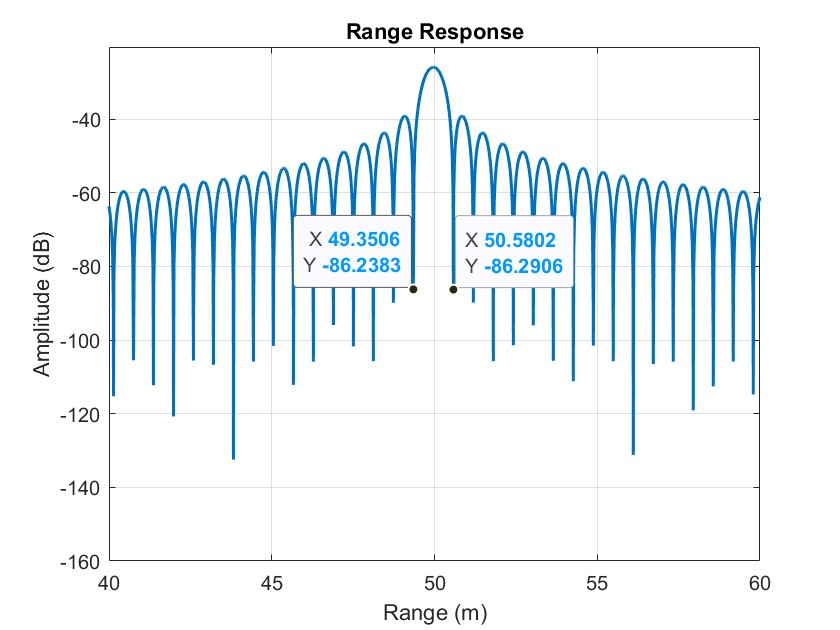
\includegraphics[width=0.8\linewidth]{802_11p_ofdm_improved_range_response_mainlobe_width.jpg}}
\caption{Updated OFDM Radar Range Response Mainlobe Width}
\label{fig::802_11p_ofdm_improved_range_response_mainlobe_width}
\end{figure}

Referring to the above figure, the mainlobe width is now 1.2296 m, which corresponds to a range resolution of 0.6148 m. It is important to note that this range resolution will further degrade after windowing is applied. However, in general, this is a much more acceptable range resolution for an automotive radar.

We can also compare the SNR of this system to the SNR of the FMCW radar. As mentioned in Equation (\ref{eq::snr_propto}), the SNR is proportional to the transmit power. For an OFDM system, the transmit power is reduced by the PAPR to ensure the amplifier operates in its linear region. This will lead to an SNR degradation of 11.8 dB with respect to an FMCW radar.

The SNR in the RDM will also be scaled by the signal processing SNR gain ($G_{sp}$). Compared to the FMCW radar, only the fast time signal processing gain will be different. If the transmitted symbols are encoded with constant amplitude modulation, then the fast time signal processing SNR gain is given as follows:

\begin{equation*}
	G_{fast} = \frac{N}{L_{fast}}
\end{equation*}

where $N$ is the number of subcarriers and $L_{fast}$ is the SNR loss due to the fast-time window. For the given system, with an 80 dB Chebyshev window the fast time SNR gain will be

\begin{equation*}
	G_{fast} \approx 587.4917
\end{equation*}

Using Equation (\ref{eq::fmcw_fast_time_snr_gain}) with a PRF of $300e6/(80 \times 16) = 234.375\ \text{kHz}$, we compute $734.504$ as the equivalent FMCW SNR gain. Note that FMCW SNR gain is greater than the OFDM Radar SNR gain by approximately $(N + L)/N$. For the specified set of parameters, that works out to be roughly 0.97 dB. Therefore, we expect to the SNR in the RDM to be approximately 13 dB lower for the JRC system than it is for the FMCW radar.

which  b other variable in the SNR equation that will change for an OFDM radar is the fast signal processing gain of an OFDM radar is given by 

the unambiguous range and velocity are less critical than they are in an FMCW radar. In other words, the OFDM radar is only able to operate well within the unambiguous range and velocity of the system.


The next plot displays the signal with the same parameter without the DC null. The pick received power is almost the same as the signal received with DC null. However, the sidelobes and noise floor shifted down significantly (average of 17 dB lower). Lower sidelobes and noise floor is crucial to some applications with high scattering noise. By including DC offset, the available bandwidth is fully utilized, leading to better spectral efficiency. Each subcarrier contributes to the total system data rate. Utilizing the DC subcarrier adds additional capacity, increasing the total throughput of the system.

\begin{figure}[H]
\centering
\fbox{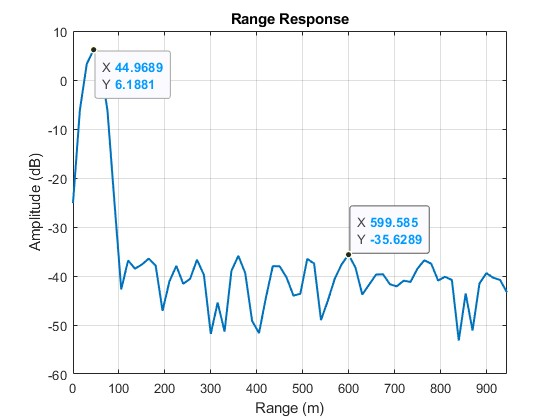
\includegraphics[width=0.8\linewidth]{OFDMRadar_No DCNull_50m}}
\caption{OFDM/Radar without DC null range plot}
\end{figure}

The previous results were simulated for a target located at 50m. We have increased the target range to 500 and 900m to see the received data quality and degradation in a long target range. As the plots indicate, in the 500m range which considers a long range for V2V radar applications, we still have a distinguishable target peak (PSLR 23dB). At 900m range the dynamic range degrades significantly to around 9dB. \par
\textbf{ Note: } For an effective presentation, we only display the analysis for signals without the DC Nulls.
\begin{figure}[H]
\centering
\fbox{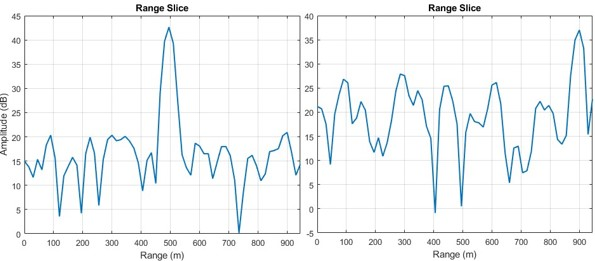
\includegraphics[width=1\linewidth]{Mix_500-900m}}
\caption{OFDM/Radar No DC null range plot 500m (left) and 900m (right)}
\end{figure} 
To ensure a fair comparison between OFDM and FMCW radar, the PSLR versus range graph is presented. Up to a range of 200 meters, the PSLR remains high at 80 dB, indicating excellent radar detection performance. Beyond 200 meters, the PSLR decreases significantly, and by approximately 1200 meters, the range becomes ambiguous.
\begin{figure}[H]
\centering
\fbox{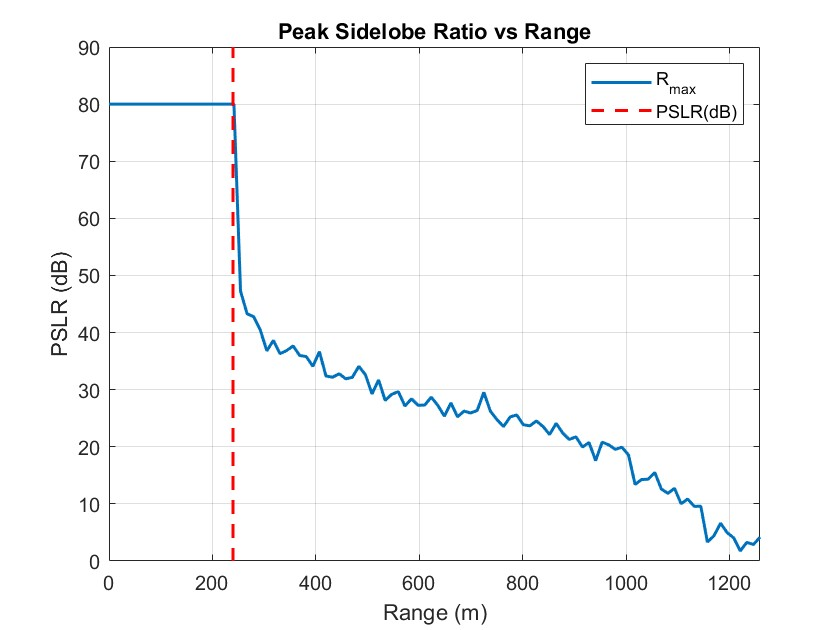
\includegraphics[width=0.8\linewidth]{OFDMRadar_PSLR vs Range}}
\caption{OFDM/Radar PSLR Measurement vs Range}
\end{figure} 
The plot below represents a Range-Doppler Map (RDM), which is a visualization used in radar systems to show the relationship between detected targets' range and relative velocity. A strong return is observed around 100 meters range and close to 50 m/s velocity. This suggests a stationary or slow-moving target with strong radar reflectivity. Other ranges (e.g., 300m, 700m) show some faint signals, but these are significantly weaker compared to the strong reflection near 100m. The resolution along the velocity axis can be further refined to detect smaller velocity variations in moving targets which can addressed by optimizing the OFDM parameter in the next step. 
\begin{figure}[H]
\centering
\fbox{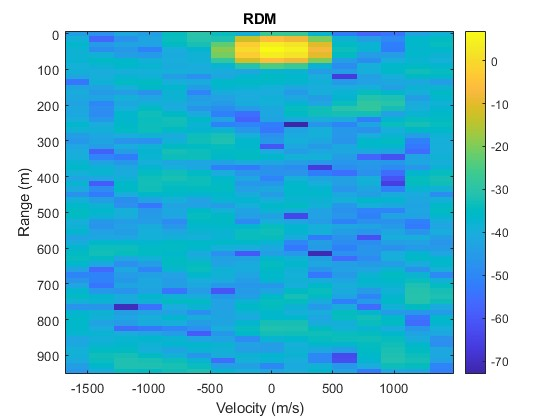
\includegraphics[width=0.8\linewidth]{OFDMRadar_RDM}}
\caption{OFDM/Radar RDM Plot}
\end{figure} 
The same PSLR vs velocity evaluation was performed for Doppler and is plotted below. It is important to note that, unlike standalone radar, the PSLR is influenced by uncompensated Doppler. The low PSLR values for Doppler make target velocity estimation challenging beyond 200 m/s.
\begin{figure}[H]
\centering
\fbox{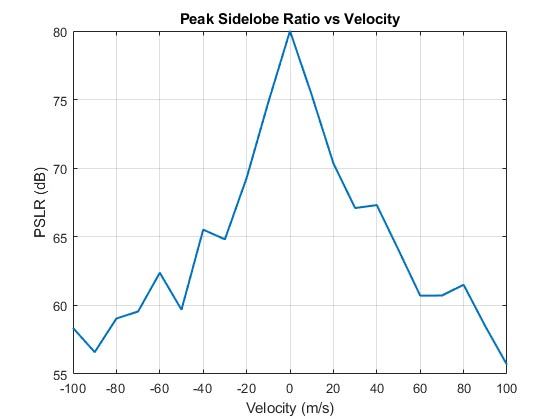
\includegraphics[width=0.8\linewidth]{OFDMRadar_PSLR vs Velocity}}
\caption{OFDM/Radar PSLR Measurement vs Velocity}
\end{figure} 

A key advantage of the OFDM technique is its flexibility to adjust parameters, enabling optimal performance tailored to the application and channel characteristics in various environments. We have adjusted the OFDM parameters to optimize radar performance while preserving high communication efficiency and capacity.
OFDM radar written in MATLAB and configured with the following set of parameters: 

\begin{center}
\begin{tabular}{|c|c|}
\hline
\textbf {Parameter} & \textbf {Value }\\
\hline
Carrier Frequency & 77 GHz \\
\hline
Sample Rate & 200 MHz \\
\hline
Number of Subcarriers & 16x64\\
\hline
Number of Data Carriers & 16x48 + 1 \\
\hline 
Number of Pilot Carriers & 16x4 \\
\hline 
Number of Pulses & 128 \\
\hline 
Target Range & 50 m \\
\hline 
Target Velocity & 50  m/s\\
\hline 
\end{tabular}
\end{center}


The graph below presents the simulation results using the parameters described above. While the noise floor has risen to 45 dB, the PSLR remains around 38 dB, similar to the unimproved simulation at a 50m range. Another significant improvement is the enhanced resolution of the detected peak, leading to more accurate range measurements.

\begin{figure}[H]
\centering
\fbox{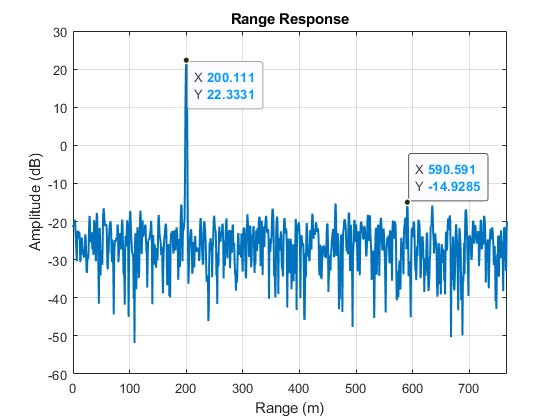
\includegraphics[width=0.8\linewidth]{OFDMRadar_No DCNull_T50_Improve}}
\caption{OFDM/Radar range plot for 50m target}
\end{figure} 
The RDM results for the given parameters, shown in the graph below, demonstrate enhanced resolution with the newly optimized OFDM parameters.
\begin{figure}[H]
\centering
\fbox{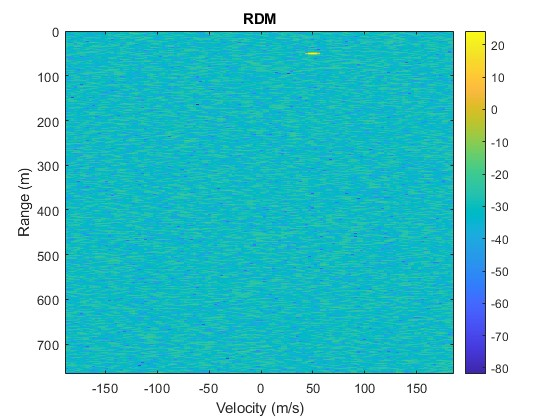
\includegraphics[width=0.8\linewidth]{OFDMRadar_RDM_Optimized}}
\caption{OFDM/Radar RDM Plot}
\end{figure} 

The parameters for the optimized OFDM yield distinct power spectral density and BER vs. SNR results. As anticipated, the total power density decreases by 20 dB, a direct consequence of the increased number of data carriers, which has been multiplied by a factor of 16 compared to OFDM stand-alone. The measured average signal power for both optimized OFDM/Radar and OFDM stand-alone are in the same range (-13 dB).

\begin{figure}[H]
\centering
\fbox{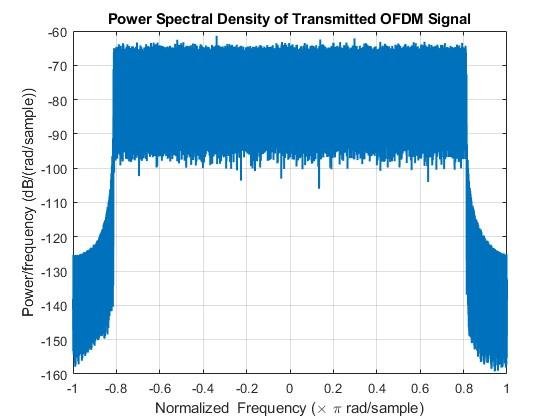
\includegraphics[width=0.8\linewidth]{Pwr Density_Optimized OFDMRadar}}
\caption{OFDM/Radar Power Spectral Density}
\end{figure} 
The final parameter compared for optimized OFDM signal integrity against stand-alone OFDM is the BER vs. SNR. The plot below shows that the BER results align with the expected values and are within the same range as those of stand-alone OFDM.
\begin{figure}[H]
\centering
\fbox{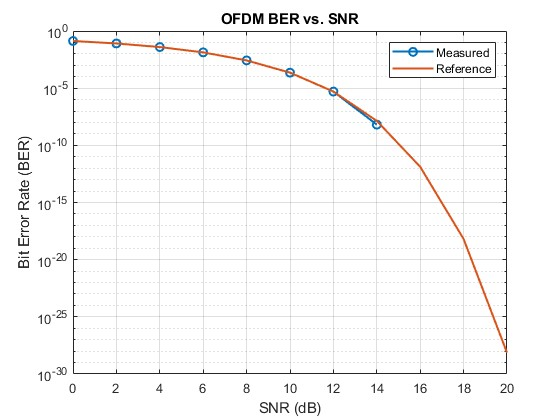
\includegraphics[width=0.8\linewidth]{BER vs SNR_Optimized OFDMRadar_AWGN}}
\caption{OFDM/Radar BER vs SNR}
\end{figure} 
\section {Conclusion}
While JRC may slightly compromise the standalone performance of either radar (resolution) or communication (capacity), it offers significant advantages in shared resource utilization, reduced hardware cost, and suitability for modern multi-functional systems like autonomous vehicles.


	\bibliographystyle {IEEEtran}
	\bibliography {References}
	
	%\nocite{yang_subcarrier_multiplexing}
	%\bibliography{sources}{}
   % \bibliographystyle{ieeetr}
  
\end{document}

